%%%%%%%%%%%%%%%%%%%%%%%%%%%%%%%%%%%%%%%%%%%%%%%%%%%%%%%%%%%%%%%%%%
%%%%%%%%%%%%%%%%%%%%%%%%%%%%%%%%%%%%%%%%%%%%%%%%%%%%%%%%%%%%%%%%%%
%\pagestyle{myheadings} \markright{Daniel Wollschläger \hfill Grundlagen der Datenanalyse mit R}
\chapter{Survival-Analyse}
\label{sec:survival}
%%%%%%%%%%%%%%%%%%%%%%%%%%%%%%%%%%%%%%%%%%%%%%%%%%%%%%%%%%%%%%%%%%
%%%%%%%%%%%%%%%%%%%%%%%%%%%%%%%%%%%%%%%%%%%%%%%%%%%%%%%%%%%%%%%%%%

\index{Ereigniszeiten|see{Survival-Analse}}
\index{Überlebenszeiten|see{Survival-Analse}}
\index{Survival-Analyse}
Die Survival-Analyse modelliert Überlebenszeiten \cite{HosmerJr2008,Klein2003}. Diese geben allgemein an, wieviel Zeit bis zum Eintreten eines bestimmten Ereignisses verstrichen ist und sollen hier deshalb gleichbedeutend mit \emph{Ereigniszeiten} sein. Es kann sich dabei etwa um die Zeitdauer handeln, die ein Patient nach einer Behandlung weiter am Leben ist, um die verstrichene Zeit, bis ein bestimmtes Bauteil im Gebrauch einen Defekt aufweist, oder um die Dauer, die ein Kleinkind benötigt, um ein vordefiniertes Entwicklungsziel zu erreichen -- z.\,B.\ einen Mindestwortschatz besitzt. Bei der Analyse von Überlebenszeiten kann sowohl die Form ihres grundsätzlichen Verlaufs von Interesse sein, als auch inwiefern ihr Verlauf systematisch von Einflussgrößen abhängt.

Die folgenden Auswertungen verwenden Funktionen des Pakets\index[pack]{survival@\lstinline{survival}} \lstinline!survival!, das im Basisumfang von R enthalten ist. Seine Anwendung wird vertiefend in \citeA{HarrellJr2001} behandelt.

%%%%%%%%%%%%%%%%%%%%%%%%%%%%%%%%%%%%%%%%%%%%%%%%%%%%%%%%%%%%%%%%%%
%%%%%%%%%%%%%%%%%%%%%%%%%%%%%%%%%%%%%%%%%%%%%%%%%%%%%%%%%%%%%%%%%%
\section{Verteilung von Ereigniszeiten}
\label{sec:survDistrib}
%%%%%%%%%%%%%%%%%%%%%%%%%%%%%%%%%%%%%%%%%%%%%%%%%%%%%%%%%%%%%%%%%%
%%%%%%%%%%%%%%%%%%%%%%%%%%%%%%%%%%%%%%%%%%%%%%%%%%%%%%%%%%%%%%%%%%

Überlebenszeiten lassen sich äquivalent durch verschiedene Funktionen beschreiben, die jeweils andere Eigenschaften ihrer Verteilung hervortreten lassen: Die Überlebenszeit selbst sei $T$ mit Werten $\geq 0$ und einer -- hier als stetig vorausgesetzten -- Dichtefunktion $f(t)$.\footnote{$f(t) = \lim_{\Delta_{t} \to 0^{+}} \frac{P(t \leq T < t + \Delta_{t})}{\Delta_{t}}$ in Abhängigkeit von der Zeit $t$ und der Intervallbreite $\Delta_{t}$.} Die zugehörige Verteilungsfunktion $F(t) = P(T \leq t)$ liefert die Wahrscheinlichkeit, mit der $T$ höchstens den Wert $t$ erreicht. Die monoton fallende Survival-Funktion $S(t) = P(T > t) = 1-F(t)$ gibt an, mit welcher Wahrscheinlichkeit die Überlebenszeit größer als $t$ ist. Dabei wird $S(0) = 1$ vorausgesetzt, zum Zeitpunkt $t = 0$ soll das Ereignis also noch nicht eingetreten sein. Schließlich drückt die \emph{Hazard}-Funktion $\lambda(t)$ die unmittelbare Ereignisrate zum Zeitpunkt $t$ aus.
\begin{equation*}
\lambda(t) = \lim_{\Delta_{t} \to 0^{+}} \frac{P(t \leq T < t + \Delta_{t} \, | \, T \geq t)}{\Delta_{t}} = \frac{P(t \leq T < t + \Delta_{t}) / \Delta_{t}}{P(T > t)} = \frac{f(t)}{S(t)}, \quad t \geq 0
\end{equation*}

$\lambda(t)$ ist bei kleiner werdender Intervallbreite $\Delta_{t}$ der Grenzwert für die bedingte Wahrscheinlichkeit pro Zeiteinheit, dass das Ereignis unmittelbar eintritt, wenn es bis zum Zeitpunkt $t$ noch nicht eingetreten ist. Bezeichnet $\# \text{Personen} \, | \, \text{Ereignis} \in [t, t + \Delta_{t})$ die Anzahl der Personen, bei denen das Ereignis im Intervall $[t, t + \Delta_{t})$ eintritt und $\# \text{Personen} \, | \, \text{Ereignis} \geq t$ die Anzahl der Personen, bei denen das Ereignis zum Zeitpunkt $t$ noch eintreten kann, lässt sich das hazard auf empirischer Ebene wie folgt formulieren:\footnote{$\# \text{Personen} \, | \, \text{Ereignis} \geq t$ ist die Größe des \emph{risk set} bzw.\ die Anzahl der Beobachtungsobjekte \emph{at risk} zum Zeitpunkt $t$.}
\begin{equation*}
\hat{\lambda}(t) = \frac{\# \text{Personen} \, | \, \text{Ereignis} \in [t, t+\Delta_{t})}{\# \text{Personen} \, | \, \text{Ereignis} \geq t} \cdot \frac{1}{\Delta_{t}}
\end{equation*}

$\hat{\lambda}(t)$ gibt also an, bei welchem Anteil verbleibender Personen ohne Ereignis bis zum Zeitpunkt $t$ das Ereignis pro Zeiteinheit eintritt. Bei Werten der monoton steigenden kumulativen Hazard-Funktion $\Lambda(t) = -\ln S(t)$ handelt es sich um das bis zum Zeitpunkt $t$ kumulierte Risiko, dass sich das Ereignis unmittelbar ereignet. Umgekehrt gilt $S(t) = \euler^{-\Lambda(t)}$.

Hazard- und Survival-Funktion bedingen einander. Nimmt man eine über die Zeit konstante Ereignisrate $\lambda(t) = \frac{1}{b}$ an (wie etwa beim radioaktiven Zerfall), impliziert dies eine exponentiell verteilte Überlebenszeit $T$ (Abschn.\ \ref{sec:survParam}). Die bedingte Wahrscheinlichkeit, dass ein noch nicht eingetretenes Ereignis unmittelbar auf $t$ folgt, wäre damit unabhängig von der bereits verstrichenen Zeit $t$. Mit der Annahme, dass die logarithmierte Ereignisrate linear von $t$ abhängt ($\ln \lambda(t) = \alpha + \rho \, t$ mit $y$-Achsenabschnitt $\alpha$ und Steigung $\rho$), ergibt sich entsprechend eine Gompertz-Verteilung von $T$. Analog führt die Annahme, dass die logarithmierte Ereignisrate linear mit der logarithmierten Zeit zusammenhängt ($\ln \lambda(t) = \alpha + \rho \ln t$), zu einer Weibull-Verteilung von $T$ (Abschn.\ \ref{sec:survParam}). Bei einem positivem $\rho$ würde in beiden Fällen das hazard mit der Zeit ansteigen, was oft in Situationen angemessen ist, in denen das Eintreten des Ereignisses mit kontinuierlichen Reifungs- oder Abnutzungsprozessen zusammenhängt.

%%%%%%%%%%%%%%%%%%%%%%%%%%%%%%%%%%%%%%%%%%%%%%%%%%%%%%%%%%%%%%%%%%
%%%%%%%%%%%%%%%%%%%%%%%%%%%%%%%%%%%%%%%%%%%%%%%%%%%%%%%%%%%%%%%%%%
\section{Zensierte und gestutzte Ereigniszeiten}
\label{sec:survData}
%%%%%%%%%%%%%%%%%%%%%%%%%%%%%%%%%%%%%%%%%%%%%%%%%%%%%%%%%%%%%%%%%%
%%%%%%%%%%%%%%%%%%%%%%%%%%%%%%%%%%%%%%%%%%%%%%%%%%%%%%%%%%%%%%%%%%

Um festzustellen, wann ein Zielereignis eintritt, werden die untersuchten Objekte über eine gewisse Zeit hinweg beobachtet -- etwa wenn bei aus einer stationären Behandlung entlassenen Patienten mit Substanzmissbrauch erhoben wird, ob sich innerhalb eines Zeitraums ein Rückfall ereignet. Meist weisen empirisch erhobene Überlebenszeiten dabei die Besonderheit auf, dass von einigen Beobachtungseinheiten die Zeit bis zum Eintreten des Ereignisses unbekannt bleibt, was spezialisierte statistische Modelle notwendig macht.

Der Erhebungszeitraum ist oft begrenzt, so dass nicht für alle Untersuchungseinheiten das Ereignis auch tatsächlich innerhalb des Beobachtungszeitraums auftritt. Für solche \emph{rechts-zensierten} Daten ist also nur bekannt, dass die Überlebenszeit den letzten Beobachtungszeitpunkt überschreitet, nicht aber ihr exakter Wert. Eine andere Ursache für rechts-zensierte Daten kann ein frühzeitiger dropout aus der Studie nach einem Umzug oder bei schwindender Motivation zur Teilnahme sein. \emph{Links-zensierte} Daten entstehen, wenn das Ereignis bekanntermaßen bereits an einem unbekannten Zeitpunkt vor Beginn der Erhebung eingetreten ist. Daten werden als \emph{links-gestutzt} bezeichnet, wenn sich das Ereignis bei manchen potentiellen Beobachtungseinheiten bereits vor Erhebungsbeginn ereignet und sie deswegen nicht mehr in der Studie berücksichtigt werden können. Während die Häufigkeit zensierter Beobachtungen in der Stichprobe bekannt ist, fehlt über gestutzte Daten jede Information.

Wichtig für die Survival-Analyse ist die Annahme, dass der zur Zensierung führende Mechanismus unabhängig von Einflussgrößen auf die Überlebenszeit ist, Beobachtungsobjekte mit zensierter Überlebenszeit also kein systematisch anderes hazard haben. Diese Bedingung wäre etwa dann erfüllt, wenn zensierte Daten dadurch entstehen, dass eine Studie zu einem vorher festgelegten Zeitpunkt endet, bis zu dem nicht bei allen Untersuchungseinheiten das Ereignis eingetreten ist. Bewirkt eine Ursache dagegen sowohl das nahe bevorstehende Eintreten des Ereignisses selbst als auch den Ausfall von Beobachtungsmöglichkeiten, wäre die Annahme nicht-informativer Zensierung verletzt. So könnte eine steigende zeitliche Beanspruchung im Beruf bei Patienten mit Substanzmissbrauch einerseits dazu führen, dass die Bereitschaft zur Teilnahme an Kontrollterminen sinkt, andererseits könnte sie gleichzeitig die Wahrscheinlichkeit eines Rückfalls erhöhen. Wenn selektiv Beobachtungseinheiten mit erhöhtem hazard nicht mehr beobachtet werden können, besteht die Gefahr verzerrter Schätzungen des Verlaufs der Überlebenszeiten.

%%%%%%%%%%%%%%%%%%%%%%%%%%%%%%%%%%%%%%%%%%%%%%%%%%%%%%%%%%%%%%%%%%
%%%%%%%%%%%%%%%%%%%%%%%%%%%%%%%%%%%%%%%%%%%%%%%%%%%%%%%%%%%%%%%%%%
\subsection{Zeitlich konstante Prädiktoren}
\label{sec:survTimeInd}
%%%%%%%%%%%%%%%%%%%%%%%%%%%%%%%%%%%%%%%%%%%%%%%%%%%%%%%%%%%%%%%%%%
%%%%%%%%%%%%%%%%%%%%%%%%%%%%%%%%%%%%%%%%%%%%%%%%%%%%%%%%%%%%%%%%%%

Survival-Daten beinhalten Angaben zum Beobachtungszeitpunkt, zu den Prädiktoren der Überlebenszeit sowie eine Indikatorvariable dafür, ob das Ereignis zum angegebenen Zeitpunkt beobachtet wurde. Für die Verwendung in späteren Analysen sind Beobachtungszeitpunkt und Indikatorvariable zunächst in einem Survival-Objekt zusammenzuführen, das Informationen zur Art der Zensierung der Daten berücksichtigt. Dies geschieht für potentiell rechts-zensierte Daten mit\index[func]{Surv()@\lstinline{Surv()}} \lstinline!Surv()! aus dem Paket\index[pack]{survival@\lstinline{survival}} \lstinline!survival! in der folgenden Form:
\begin{lstlisting}
Surv(<<Zeitpunkt>>, <<Status>>)
\end{lstlisting}

Als erstes Argument ist ein Vektor der Zeitpunkte $t_{i} > 0$ zu nennen, an denen das Ereignis bei den Objekten $i$ eingetreten ist. Bei rechts-zensierten Beobachtungen ist dies der letzte bekannte Zeitpunkt, zu dem das Ereignis noch nicht eingetreten war. Die dabei implizit verwendete Zeitskala hat ihren Ursprung $0$ beim Eintritt in die Untersuchung. Das zweite Argument ist eine numerische oder logische Indikatorvariable, die den Status zu den genannten Zeitpunkten angibt -- ob das Ereignis also vorlag ($1$ bzw.\ \lstinline!TRUE!) oder nicht ($0$ bzw.\ \lstinline!FALSE! bei rechts-zensierten Beobachtungen).\footnote{Für Intervall-zensierte Daten vgl.\ \lstinline!?Surv!. Vergleiche Abschn.\ \ref{sec:survTimeDep} für zeitabhängige Prädiktoren und Fälle, in denen mehrere Ereignisse pro Beobachtungsobjekt möglich sind.}

Für die folgende Simulation von Überlebenszeiten soll eine Weibull-Verteilung mit Annahme proportionaler hazards bzgl.\ der Einflussfaktoren (Abschn.\ \ref{sec:survCPH}) zugrunde gelegt werden (Abb.\ \ref{fig:survivalT}). Dafür sei der lineare Effekt der Einflussgrößen durch $\bm{X} \bm{\beta} = \beta_{1} X_{1} + \dots + \beta_{j} X_{j} + \dots + \beta_{p} X_{p}$ gegeben (ohne absoluten Term $\beta_{0}$, s.\ Abschn.\ \ref{sec:multALMregr}). Hier soll dafür ein kontinuierlicher Prädiktor sowie eine kategoriale UV mit $3$ Stufen verwendet werden, wobei beide Variablen nicht über die Zeit variieren. Zusätzlich sei die Schichtung hinsichtlich des Geschlechts berücksichtigt.
\begin{lstlisting}
> N   <- 180                                 # Anzahl Personen
> P   <- 3                                   # Anzahl Stufen UV
> sex <- factor(sample(c("f", "m"), N, replace=TRUE))     # Geschlecht
> X   <- rnorm(N, 0, 1)                      # kontinuierl. Prädiktor
> IV  <- factor(rep(LETTERS[1:P], each=N/P)) # UV Faktor

# Effekte der UV-Stufen: 1. Stufe = baseline -> Effekt 0
> IVeff <- c(0, -1, 1.5)

# zusammengefasster Effekt der Einflussgrößen mit zufälligem Fehler
> Xbeta <- 0.7*X + IVeff[unclass(IV)] + rnorm(N, 0, 2)
\end{lstlisting}

Weiter sei $U \sim \mathcal{U}(0, 1)$ eine gleichverteilte Zufallsvariable auf dem Intervall $[0, 1]$. Weibull-verteilte Überlebenszeiten können dann als Realisierung von $T = (-\ln(U) \, b^{a} \, \euler^{-\bm{X} \bm{\beta}})^{\frac{1}{a}}$ simuliert werden (Abschn.\ \ref{sec:survParam}). Die hier getroffene Wahl $a = 1.5$ führt dazu, dass $\ln \lambda(t)$ linear mit $\ln t$ ansteigt. Die Simulation von Überlebenszeiten mit anderen kumulativen Hazard-Funktionen $\Lambda(t)$ unter Annahme proportionaler hazards erfolgt allgemein mit $\Lambda^{-1}(-\ln(U) \, \euler^{-\bm{X} \bm{\beta}})$ \cite{Bender2005}.
\begin{lstlisting}
# Weibull-Verteilung zur Charakterisierung des baseline-hazards
> weibA <- 1.5                               # Formparameter
> weibB <- 100                               # Skalierungsparameter
> U     <- runif(N, 0, 1)                    # gleichverteilte Variable

# Überlebenszeiten - aufrunden für t > 0
> eventT <- ceiling((-log(U)*(weibB^weibA)*exp(-Xbeta))^(1/weibA))
> obsLen <- 120                              # Beobachtungsdauer

# stelle kumulierte Verteilung der Überlebenszeiten dar
> plot(ecdf(eventT), xlim=c(0, 200), main="Kumulative
+      Überlebenszeit-Verteilung", xlab="t", ylab="F(t)")

> abline(v=obsLen, col="blue", lwd=2)        # Untersuchungsende
> text(obsLen-5, 0.2, adj=1, labels="Ende Beobachtungszeit")
\end{lstlisting}

\begin{figure}[ht]
\centering
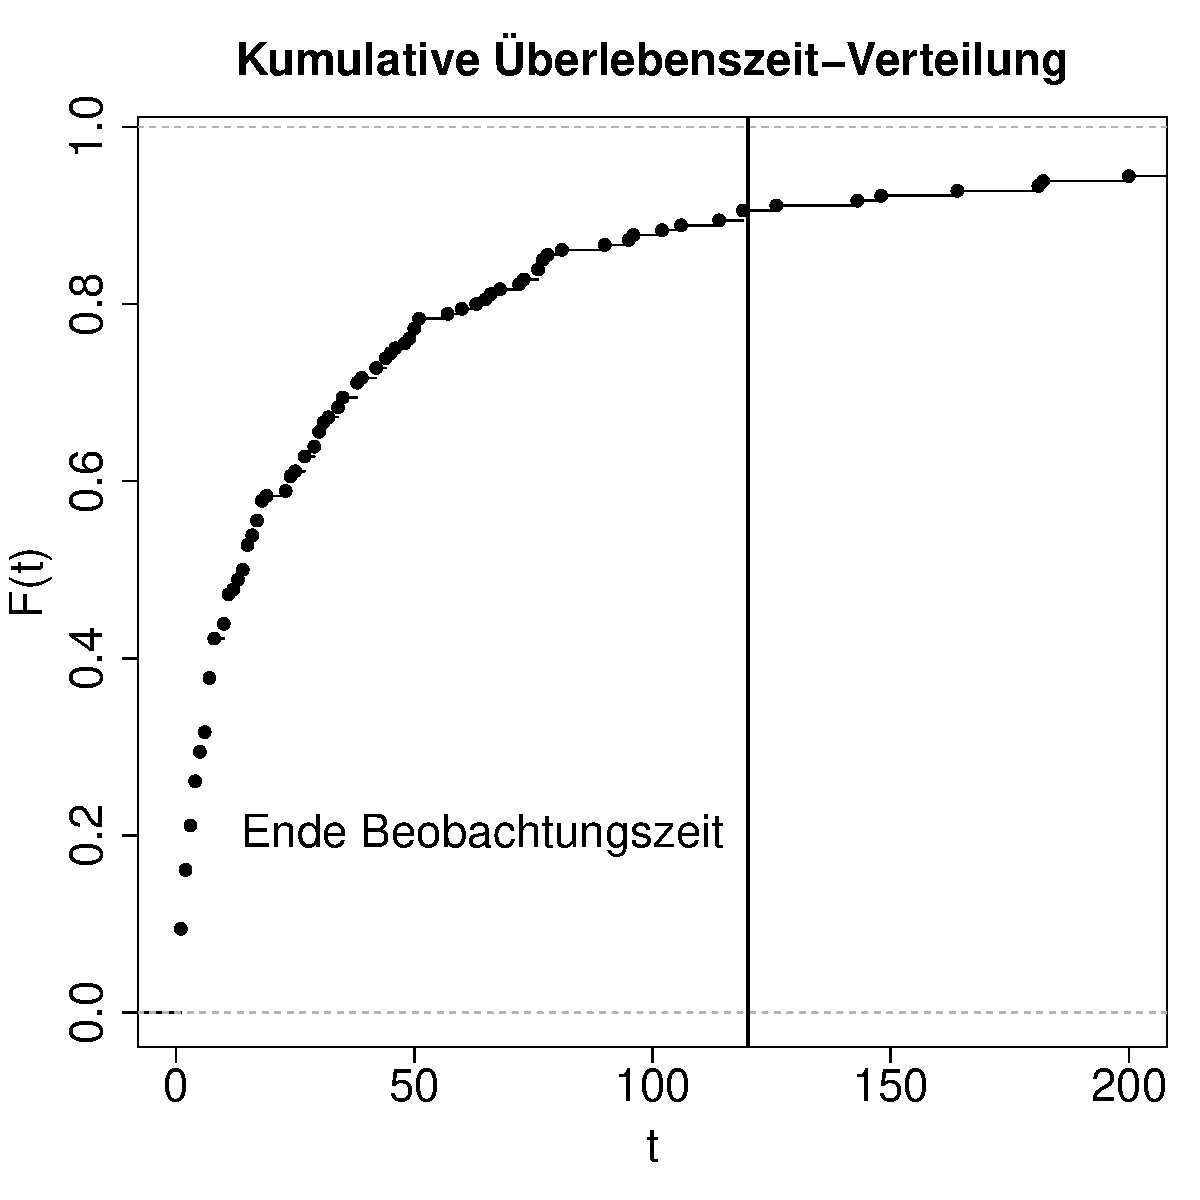
\includegraphics[width=8cm]{survivalT}
\vspace*{-1em}
\caption{Kumulative Verteilung simulierter Survival-Daten mit Weibull-Verteilung}
\label{fig:survivalT}
\end{figure}

Der zur rechts-Zensierung führende Prozess soll hier ausschließlich das geplante Ende des Beobachtungszeitraums sein. Alle nach dem Endpunkt der Erhebung liegenden Überlebenszeiten werden daher auf diesen Endpunkt zensiert. Entsprechend wird das Ereignis nur beobachtet, wenn die Überlebenszeit nicht nach dem Endpunkt liegt.
\begin{lstlisting}
> censT  <- rep(obsLen, N)                       # Zensierungszeit
> obsT   <- pmin(eventT, censT)         # zensierte Überlebenszeit
> status <- eventT <= censT                      # Ereignis-Status
> dfSurv <- data.frame(obsT, status, sex, X, IV) # Datensatz
> library(survival)                              # für Surv()
> Surv(obsT, status)                             # Survival-Objekt
[1] 63 25 73 120+ 4 39 4 1 10 11 2 120+ 7 29 95  # ...
\end{lstlisting}

In der (hier gekürzten) Ausgabe des mit \lstinline!Surv()! gebildeten Survival-Objekts sind zensierte Überlebenszeiten durch ein $+$ kenntlich gemacht.

%%%%%%%%%%%%%%%%%%%%%%%%%%%%%%%%%%%%%%%%%%%%%%%%%%%%%%%%%%%%%%%%%%
%%%%%%%%%%%%%%%%%%%%%%%%%%%%%%%%%%%%%%%%%%%%%%%%%%%%%%%%%%%%%%%%%%
\subsection{Daten in Zählprozess-Darstellung}
\label{sec:survTimeDep}
%%%%%%%%%%%%%%%%%%%%%%%%%%%%%%%%%%%%%%%%%%%%%%%%%%%%%%%%%%%%%%%%%%
%%%%%%%%%%%%%%%%%%%%%%%%%%%%%%%%%%%%%%%%%%%%%%%%%%%%%%%%%%%%%%%%%%

\index{Survival-Analyse!Zählprozess-Darstellung}
Überlebenszeiten lassen sich samt der zugehörigen Werte für relevante Prädiktoren auch in der \emph{Zählprozess}-Darstellung notieren. Für jedes Beobachtungsobjekt unterteilt diese Darstellung die Zeit in diskrete Intervalle $(\text{Start}, \text{Stop}]$, für die jeweils angegeben wird, ob sich ein Ereignis im Intervall ereignet hat. Die Intervalle sind links offen und rechts geschlossen, zudem muss $\text{Stop} > \text{Start}$ gelten, so dass keine Intervalle der Länge $0$ auftauchen. Der Aufruf von \lstinline!Surv()! erweitert sich dafür wie folgt:
\begin{lstlisting}
Surv(<<Start>>, <<Stop>>, <<Status>>)
\end{lstlisting}

\lstinline!<<Start>>! gibt den Beginn eines Beobachtungsintervalls an. \lstinline!<<Stop>>! ist wieder der beobachtete Ereignis-Zeitpunkt bzw.\ bei rechts-zensierten Daten der letzte bekannte Zeitpunkt, zu dem kein Ereignis vorlag. Intervalle für unterschiedliche Personen dürfen dabei unterschiedliche Grenzen besitzen. Anders als in der in Abschn.\ \ref{sec:survTimeInd} vorgestellten Darstellung kann die hier implizit verwendete Zeitskala flexibel etwa das Alter eines Beobachtungsobjekts sein, die (vom Eintritt in die Untersuchung abweichende) Zeit seit einer Diagnose oder die absolute kalendarische Zeit. Ist das Ereignis im Intervall $(\text{Start}, \text{Stop}]$ eingetreten, ist \lstinline!<<Status>>! gleich $1$ (bzw.\ \lstinline!TRUE!), sonst $0$ (bzw.\ \lstinline!FALSE! bei rechts-zensierten Beobachtungen).

Durch die explizite Angabe des Beginns eines Beobachtungszeitraums gibt die Zählprozess-Darstellung Auskunft darüber, vor welchem Zeitpunkt keine Informationen darüber vorliegen, ob sich das Ereignis bereits einmal ereignet hat. Die Darstellungsform ist damit für links-gestutzte Daten geeignet. Tabelle \ref{tab:survLeftCens} zeigt die Darstellung am Beispiel von vier Beobachtungsobjekten aus zwei Gruppen, deren Lebensalter zu Beginn und zu Ende einer zehnjährigen Untersuchung ebenso erfasst wurde wie der Ereignis-Status zu Ende der Untersuchung.

\begin{table}[ht]
\centering
\caption{Zählprozess-Darstellung für vier links-gestutzte und teilweise rechts-zensierte Beobachtungen mit Überlebenszeiten (Lebensalter) $\{47, 38^{+}, 41, 55\}$ aus zwei Gruppen in einer zehnjährigen Untersuchung}
\label{tab:survLeftCens}
\begin{tabular}{llll}
\hline
\sffamily Start & \sffamily Stop & \sffamily Gruppe & \sffamily Status\\\hline\hline
37              & 47             & Treatment        & 1 \\
28              & 38             & Treatment        & 0 \\
31              & 41             & Control          & 1 \\
45              & 55             & Control          & 1 \\\hline
\end{tabular}
\end{table}

Die Zählprozess-Darstellung erlaubt es auch Erhebungssituationen abzubilden, in denen der Status von Beobachtungsobjekten
an mehreren Zeitpunkten $t_{m}$ ermittelt wird. So könnte etwa bei regelmäßigen Kontrollterminen nach einer Operation geprüft werden, ob eine bestimmte Krankheit wieder diagnostizierbar ist. Der Aufruf von \lstinline!Surv()! hat dann die Form wie bei links-gestutzten Beobachtungen, wobei pro Beobachtungsobjekt mehrere $(\text{Start}, \text{Stop}]$ Intervalle vorliegen. Für den Untersuchungszeitpunkt $t_{m}$ ist dabei \lstinline!<<Start>>! der letzte zuvor liegende Untersuchungszeitpunkt $t_{m-1}$, während \lstinline!<<Stop>>! $t_{m}$ selbst ist. Für den ersten Untersuchungszeitpunkt $t_{1}$ ist $t_{0}$ der Eintritt in die Untersuchung, etwa das zugehörige kalendarische Datum oder das Alter eines Beobachtungsobjekts.

%%%%%%%%%%%%%%%%%%%%%%%%%%%%%%%%%%%%%%%%%%%%%%%%%%%%%%%%%%%%%%%%%%
%%%%%%%%%%%%%%%%%%%%%%%%%%%%%%%%%%%%%%%%%%%%%%%%%%%%%%%%%%%%%%%%%%
\subsubsection{Wiederkehrende Ereignisse}
%%%%%%%%%%%%%%%%%%%%%%%%%%%%%%%%%%%%%%%%%%%%%%%%%%%%%%%%%%%%%%%%%%
%%%%%%%%%%%%%%%%%%%%%%%%%%%%%%%%%%%%%%%%%%%%%%%%%%%%%%%%%%%%%%%%%%

\index{Survival-Analyse!wiederkehrende Ereignisse}
Da der Ereignis-Status in der Zählprozess-Darstellung am Ende mehrerer Zeitintervalle erfasst werden kann, ist es auch möglich Ereignisse abzubilden, die sich pro Untersuchungseinheit potentiell mehrfach ereignen. Die spätere Analyse wiederkehrender Ereignisse muss dabei berücksichtigen, ob diese unabhängig voneinander eintreten, oder etwa in ihrer Reihenfolge festgelegt sind.

Bei mehreren Beobachtungszeitpunkten muss der Datensatz für die Zählprozess-Darstellung im Long-Format vorliegen, d.\,h.\ für jede Untersuchungseinheit mehrere Zeilen umfassen (Abschn.\ \ref{sec:reshape}). Pro Beobachtungszeitpunkt $t_{m}$ ist für jede Untersuchungseinheit eine Zeile mit den Werten $t_{m-1}$, $t_{m}$, den Werten der Prädiktoren sowie dem Ereignis-Status zu $t_{m}$ in den Datensatz aufzunehmen. Zusätzlich sollte jede Zeile den Wert eines Faktors \lstinline!<<ID>>! enthalten, der das Beobachtungsobjekt identifiziert (Tab.\ \ref{tab:survRecur}).

\begin{table}[ht]
\centering
\caption{Zählprozess-Darstellung für zwei Beobachtungsobjekte aus zwei Gruppen am Ende von je drei zweijährigen Beobachtungsintervallen mit potentiell mehrfach auftretenden Ereignissen}
\label{tab:survRecur}
\begin{tabular}{lllllll}
\hline
ID & \sffamily Start ($t_{m-1})$ & \sffamily Stop ($t_{m})$ & \sffamily Gruppe & \sffamily Status\\\hline\hline
 1 & 37      & 39        & Treatment        & 0 \\
 1 & 39      & 41        & Treatment        & 1 \\
 1 & 41      & 43        & Treatment        & 1 \\
 2 & 28      & 30        & Control          & 0 \\
 2 & 30      & 32        & Control          & 1 \\
 2 & 32      & 34        & Control          & 0 \\\hline
\end{tabular}
\end{table}

Liegen die Daten im \lstinline!(<<Zeitpunkt>>, <<Status>>)!-Format vor, können sie mit\index[func]{survSplit()@\lstinline{survSplit()}} \lstinline!survSplit()! aus dem Paket\index[pack]{survival@\lstinline{survival}} \lstinline!survival! in Zählprozess-Darstellung mit mehreren Zeitintervallen pro Beobachtungsobjekt gebracht werden.
\begin{lstlisting}
survSplit(<<Modellformel>>, cut=<<Grenzen>>, start="<<Name>>",
          id="<<Name>>", zero=<<Startzeit>>, data=<<Datensatz>>)
\end{lstlisting}

Als erstes Argument ist eine Modellformel zu übergeben, deren linke Seite ein mit \lstinline!Surv()! erstelltes Objekt ist (Abschn.\ \ref{sec:survData}). Die rechte Seite der Modellformel definiert die Variablen, die im erstellten Datensatz beibehalten werden -- meist \lstinline!.! stellvertretend für alle Variablen des Datensatzes \lstinline!data!. \lstinline!cut! legt die linken Grenzen $t_{m-1}$ der neu zu bildenden Intervalle fest, jedoch ohne die erste Grenze $t_{0}$.\footnote{Bei nicht wiederkehrenden Ereignissen ist die Einteilung der Gesamtbeobachtungszeit in einzelne, bündig aneinander anschließende Intervalle beliebig: Die einzelne Beobachtung im \lstinline!(<<Zeitpunkt>>, <<Status>>)!-Format \lstinline!(10, TRUE)! ist sowohl äquivalent zu den zwei Beobachtungen in Zählprozess-Darstellung \lstinline!(0, 4, FALSE)!, \lstinline!(4, 10, TRUE)! als auch zu den drei Beobachtungen \lstinline!(0, 2, FALSE)!, \lstinline!(2, 6, FALSE)!, \lstinline!(6, 10, TRUE)!.} \lstinline!start! ist der Name der zu erstellenden Variable der linken Intervallgrenzen $t_{m-1}$. Soll eine Variable hinzugefügt werden, die jedem Intervall das zugehörige Beobachtungsobjekt zuordnet, muss deren Name für \lstinline!id! genannt werden. Mit \lstinline!zero! lässt sich in Form eines Vektors oder als -- dann für alle Beobachtungen identische -- Zahl angeben, was der Zeitpunkt $t_{0}$ des Beginns der Beobachtungen ist.
\begin{lstlisting}
> library(survival)                             # für survSplit()
> dfSurvCP <- survSplit(Surv(obsT, status) ~ ., cut=seq(30, 90, by=30),
+                       start="start", id="ID", zero=0, data=dfSurv)

# sortiere nach Beobachtungsobjekt und linken Intervallgrenzen
> idxOrd <- order(dfSurvCP$ID, dfSurvCP$start)
> head(dfSurvCP[idxOrd, ], n=7)
  sex          X IV ID start obsT status
1   f -1.3130607  A  1     0   30      0
2   f -1.3130607  A  1    30   60      0
3   f -1.3130607  A  1    60   63      1
4   m -0.1384786  A  2     0   25      1
5   m -0.3846335  A  3     0   30      0
6   m -0.3846335  A  3    30   60      0
7   m -0.3846335  A  3    60   73      1
\end{lstlisting}

%%%%%%%%%%%%%%%%%%%%%%%%%%%%%%%%%%%%%%%%%%%%%%%%%%%%%%%%%%%%%%%%%%
%%%%%%%%%%%%%%%%%%%%%%%%%%%%%%%%%%%%%%%%%%%%%%%%%%%%%%%%%%%%%%%%%%
\subsubsection{Zeitabhängige Prädiktoren}
%%%%%%%%%%%%%%%%%%%%%%%%%%%%%%%%%%%%%%%%%%%%%%%%%%%%%%%%%%%%%%%%%%
%%%%%%%%%%%%%%%%%%%%%%%%%%%%%%%%%%%%%%%%%%%%%%%%%%%%%%%%%%%%%%%%%%

\index{Survival-Analyse!zeitabhängige Prädiktoren}
In der Zählprozess-Darstellung ist es möglich, die Werte von zeitlich variablen Prädiktoren in die Daten aufzunehmen (Tab.\ \ref{tab:survTimeDep}). Eine spätere Analyse setzt dabei voraus, dass der Wert eines zeitabhängigen Prädiktors zum Zeitpunkt $t_{m}$ nur Informationen widerspiegelt, die bis $t_{m}$ vorlagen -- aber nicht später. Eine zeitlich rückwirkende Kategorisierung von Untersuchungseinheiten in verschiedene Gruppen auf Basis ihres Verhaltens zu Studienende wäre etwa demnach unzulässig. Ebenso sind meist zeitabhängige Variablen problematisch, die weniger Einflussgröße bzw.\ Prädiktor, sondern eher Effekt oder Indikator eines Prozesses sind, der zu einem bevorstehenden Ereignis führt.
% Beispiel

\begin{table}[ht]
\centering
\caption{Zählprozess-Darstellung für zeitabhängige Prädiktoren bei drei Beobachtungsobjekten mit Überlebenszeiten $\{3, 4^{+}, 2\}$}
\label{tab:survTimeDep}
\begin{tabular}{lllll}
\hline
ID & \sffamily Start ($t_{m-1})$ & \sffamily Stop ($t_{m})$ & \sffamily Temperatur & \sffamily Status\\\hline\hline
 1 & 0       & 1       & 45                   & 0 \\
 1 & 1       & 2       & 52                   & 0 \\
 1 & 2       & 3       & 58                   & 1 \\
 2 & 0       & 1       & 37                   & 0 \\
 2 & 1       & 2       & 41                   & 0 \\
 2 & 2       & 3       & 56                   & 0 \\
 2 & 3       & 4       & 57                   & 0 \\
 3 & 0       & 1       & 35                   & 0 \\
 3 & 1       & 2       & 61                   & 1 \\\hline
\end{tabular}
\end{table}

%%%%%%%%%%%%%%%%%%%%%%%%%%%%%%%%%%%%%%%%%%%%%%%%%%%%%%%%%%%%%%%%%%
%%%%%%%%%%%%%%%%%%%%%%%%%%%%%%%%%%%%%%%%%%%%%%%%%%%%%%%%%%%%%%%%%%
\section{Kaplan-Meier-Analyse}
\label{sec:survKM}
%%%%%%%%%%%%%%%%%%%%%%%%%%%%%%%%%%%%%%%%%%%%%%%%%%%%%%%%%%%%%%%%%%
%%%%%%%%%%%%%%%%%%%%%%%%%%%%%%%%%%%%%%%%%%%%%%%%%%%%%%%%%%%%%%%%%%

\index{Survival-Analyse!Kaplan-Meier}

%%%%%%%%%%%%%%%%%%%%%%%%%%%%%%%%%%%%%%%%%%%%%%%%%%%%%%%%%%%%%%%%%%
%%%%%%%%%%%%%%%%%%%%%%%%%%%%%%%%%%%%%%%%%%%%%%%%%%%%%%%%%%%%%%%%%%
\subsection{Survival-Funktion schätzen}
\label{sec:survKMfit}
%%%%%%%%%%%%%%%%%%%%%%%%%%%%%%%%%%%%%%%%%%%%%%%%%%%%%%%%%%%%%%%%%%
%%%%%%%%%%%%%%%%%%%%%%%%%%%%%%%%%%%%%%%%%%%%%%%%%%%%%%%%%%%%%%%%%%

Die Kaplan-Meier-Analyse liefert als nonparametrische Maximum-Likelihood-Schätzung der Survival-Funktion eine Stufenfunktion $\hat{S}(t)$, deren Stufen bei den empirisch beobachteten Ereignis-Zeitpunkten $t_{i}$ liegen. Sie wird samt der punktweisen Konfidenzintervalle mit\index[func]{survfit()@\lstinline{survfit()}} \lstinline!survfit()! aus dem Paket\index[pack]{survival@\lstinline{survival}} \lstinline!survival! berechnet.
\begin{lstlisting}
survfit(<<Modellformel>>, type="kaplan-meier", conf.type="<<CI-Typ>>")
\end{lstlisting}

Als erstes Argument ist eine Modellformel zu übergeben, deren linke Seite ein mit \lstinline!Surv()! erstelltes Objekt ist (Abschn.\ \ref{sec:survData}). Die rechte Seite der Modellformel ist entweder der konstante Term $1$ für eine globale Anpassung, oder besteht aus (zeitlich konstanten) Faktoren. In diesem Fall resultiert für jede Faktorstufe bzw.\ Kombination von Faktorstufen $g$ eine separate Schätzung $\hat{S}_{g}(t)$. Das Argument \lstinline!type! ist bei der Voreinstellung \lstinline!"kaplan-meier"! zu belassen. Mit \lstinline!conf.type! wird die Transformation für $S(t)$ angegeben, auf deren Basis die nach zugehöriger Rücktransformation gewonnenen Konfidenzintervalle für $S(t)$ konstruiert sind: Mit \lstinline!"plain"! erhält man Intervalle auf Basis von $S(t)$ selbst. Geeigneter sind oft die durch \lstinline!"log"! erzeugten Intervalle, die auf dem kumulativen hazard $\Lambda(t) = -\ln S(t)$ basieren. Mit \lstinline!"log-log"! ergeben sich die Intervalle aus dem logarithmierten kumulativen hazard $\ln \Lambda(t) = \ln (-\ln S(t))$. Auf \lstinline!"none"! gesetzt unterbleibt die Berechnung von Konfidenzintervallen.
\begin{lstlisting}
# Schätzung von S(t) ohne Trennung nach Gruppen
> library(survival)                             # für survfit()
> KM0 <- survfit(Surv(obsT, status) ~ 1,  type="kaplan-meier",
+                conf.type="log", data=dfSurv)

# Schätzung von S(t) getrennt nach Gruppen
> (KM <- survfit(Surv(obsT, status) ~ IV, type="kaplan-meier",
+                conf.type="log", data=dfSurv))
     records n.max n.start events median 0.95LCL 0.95UCL
IV=A      60    60      60     55   13.5       8      31
IV=B      60    60      60     49   33.0      17      50
IV=C      60    60      60     59    5.5       4      11
\end{lstlisting}

Die Ausgabe gibt -- ggf.\ getrennt für jede Gruppe -- Auskunft über die Anzahl der Beobachtungen (\lstinline!records!), die Anzahl der Ereignisse (\lstinline!events!) und unter \lstinline!median! eine Schätzung für den Median der Überlebenszeit (das $50 \%$-Quantil der geschätzten Survival-Funktion $\hat{S}(t)$) gefolgt von den Grenzen des zugehörigen Konfidenzintervalls (\lstinline!0.95LCL!, \lstinline!0.95UCL!). Das zurückgegebene Objekt enthält u.\,a.\ in den Komponenten \lstinline!time! die Ereignis-Zeitpunkte, in \lstinline!surv! die geschätzte Überlebensfunktion $\hat{S}(t)$ und in \lstinline!cumhaz! das geschätzte kumulative hazard $\hat{\Lambda}(t) = -\ln \hat{S}(t)$.

Analog zum geschätzten Median der Überlebenszeit ermittelt\index[func]{quantile()@\lstinline{quantile()}} \lstinline!quantile(<<survfit-Objekt>>, probs=<<Quantile>>)! beliebige Quantile von $\hat{S}(t)$ -- also Schätzungen für die Zeitpunkte, zu denen bei einem bestimmten Anteil der Beobachtungsobjekte ein Ereignis aufgetreten ist. In der Voreinstellung \lstinline!conf.int=TRUE! erhält man zusätzlich die Grenzen des jeweiligen Konfidenzintervalls für ein Quantil.
\begin{lstlisting}
# Quantile der Überlebenszeit mit Grenzen der Konfidenzintervalle
> quantile(KM0, probs=c(0.25, 0.5, 0.75), conf.int=TRUE)
$quantile
25%  50%  75%
4.0 14.5 47.0

$lower
25%  50%  75%
  3   10   35

$upper
25%  50%  75%
 7    19   68
\end{lstlisting}

Über \lstinline!print(<<survfit-Objekt>>, print.rmean=TRUE)! erhält man auch die geschätzte mittlere Überlebenszeit.
\begin{lstlisting}
> print(KM0, print.rmean=TRUE)
     n  events *rmean *se(rmean) median 0.95LCL 0.95UCL
180.00  163.00  32.64       2.89  14.50   10.00   19.00
* restricted mean with upper limit = 120
\end{lstlisting}

\lstinline!summary(<<survfit-Objekt>>, times=<<Vektor>>)! gibt detailliert Auskunft über die Werte von $\hat{S}(t)$ zu den unter \lstinline!times! genannten Zeiten $t$. So lässt sich etwa das geschätzte 100-Tage Überleben berechnen. Fehlt \lstinline!times!, umfasst die Ausgabe alle tatsächlich aufgetretenen Ereignis-Zeitpunkte $t_{i}$.
\begin{lstlisting}
# Werte der geschätzten Survival-Funktion für 20, 50, 100 Tage
> summary(KM0, times=c(20, 50, 100))       # ohne Trennung nach Gruppen
 time n.risk n.event survival std.err lower 95% CI upper 95% CI
   20     75     105    0.417  0.0367       0.3505        0.495
   50     43      34    0.228  0.0313       0.1741        0.298
  100     22      19    0.122  0.0244       0.0826        0.181
\end{lstlisting}

Die Ausgabe nennt unter \lstinline!time! die vorgegebenen Ereignis-Zeitpunkte $t_{i}$ und unter \lstinline!n.risk! die Anzahl der Personen, von denen bekannt ist, dass sie jeweils vor $t_{i}$ noch kein Ereignis hatten aber noch unter Beobachtung sind. Unter \lstinline!n.event! ist die Anzahl der Ereignisse zu $t_{i}$ aufgeführt, unter \lstinline!survival! die Schätzung $\hat{S}(t_{i})$, unter \lstinline!std.err! die geschätzte Streuung des Schätzers $\hat{S}(t_{i})$ sowie in den letzten beiden Spalten die Grenzen des punktweisen Konfidenzintervalls für $\hat{S}(t_{i})$.

%%%%%%%%%%%%%%%%%%%%%%%%%%%%%%%%%%%%%%%%%%%%%%%%%%%%%%%%%%%%%%%%%%
%%%%%%%%%%%%%%%%%%%%%%%%%%%%%%%%%%%%%%%%%%%%%%%%%%%%%%%%%%%%%%%%%%
\subsection{Survival, kumulative Inzidenz und kumulatives hazard darstellen}
%%%%%%%%%%%%%%%%%%%%%%%%%%%%%%%%%%%%%%%%%%%%%%%%%%%%%%%%%%%%%%%%%%
%%%%%%%%%%%%%%%%%%%%%%%%%%%%%%%%%%%%%%%%%%%%%%%%%%%%%%%%%%%%%%%%%%

Die grafische Darstellung von $\hat{S}(t)$ mit \lstinline!plot(<<survfit-Objekt>>)! (Abb.\ \ref{fig:survivalKM}) zeigt zusätzlich die Konfidenzintervalle. Die geschätzte kumulative Inzidenz $1-\hat{S}(t)$ erhält man mit dem Argument \lstinline!fun=function(x) { 1-x }!. Für das geschätzte kumulative hazard ist beim Aufruf von \lstinline!plot()! das Argument \lstinline!fun="cumhaz"! zu verwenden.
\begin{lstlisting}
> plot(KM0, main=expression(paste("KM-Schätzer ", hat(S)(t),
+      " mit CI")), xlab="t", ylab="Survival", lwd=2)

> plot(KM0, main=expression(paste("KM-Schätzer 1-", hat(S)(t),
+                                 " mit CI")), xlab="t",
+      ylab="kumulative Inzidenz", fun=function(x) {1-x}, lwd=2)

> plot(KM, main=expression(paste("KM-Schätzer ", hat(S)[g](t), lty=1:3,
+      " für Gruppen")), xlab="t", ylab="Survival", lwd=2, col=1:3)

> legend(x="topright", lty=1:3, col=1:3, lwd=2, legend=LETTERS[1:3])

> plot(KM0, main=expression(paste("KM-Schätzer ", hat(Lambda)(t))),
+      xlab="t", ylab="kumulatives hazard", fun="cumhaz", lwd=2)
\end{lstlisting}

\begin{figure}[!ht]
\centering
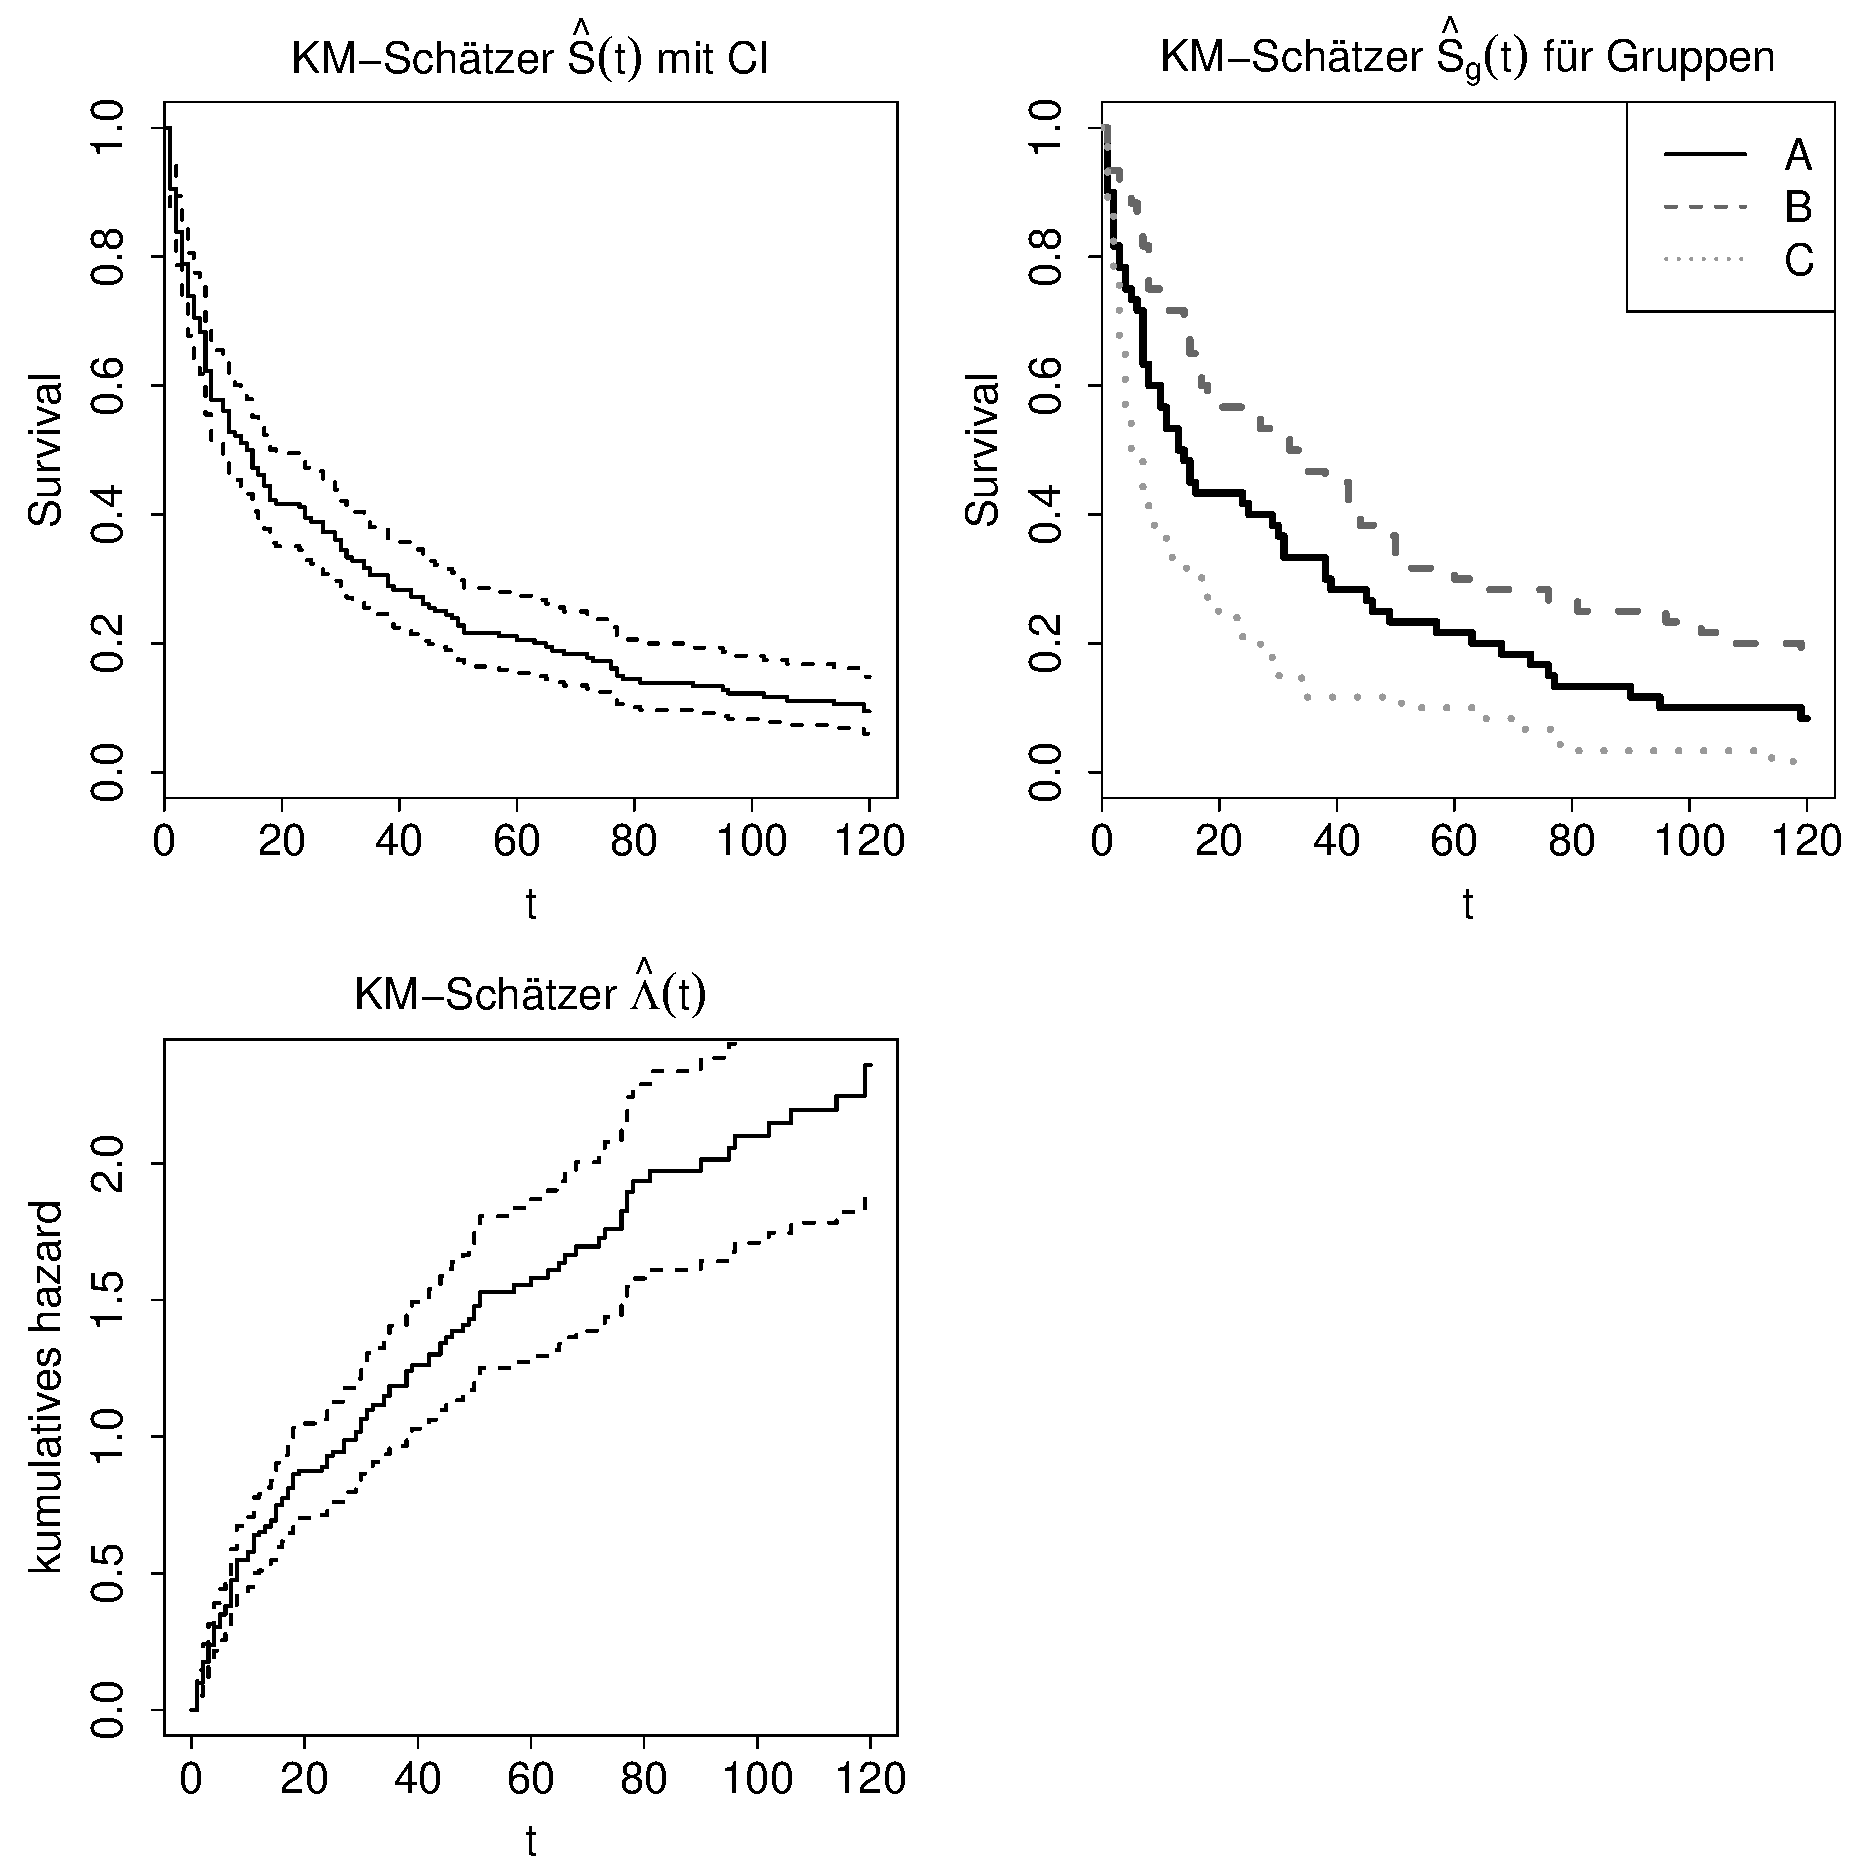
\includegraphics[width=12.5cm]{survivalKM}
\vspace*{-1em}
\caption{Kaplan-Meier-Schätzungen: Survival-Funktion $\hat{S}(t)$ sowie kumulative Inzidenz $1-\hat{S}(t)$ ohne Berücksichtigung der Gruppen (mit Konfidenzintervallen), separate Schätzungen $\hat{S}_{g}(t)$ getrennt nach Gruppen $g$ sowie die geschätzte kumulative Hazard-Funktion $\hat{\Lambda}(t)$ (mit Konfidenzintervallen)}
\label{fig:survivalKM}
\end{figure}

%%%%%%%%%%%%%%%%%%%%%%%%%%%%%%%%%%%%%%%%%%%%%%%%%%%%%%%%%%%%%%%%%%
%%%%%%%%%%%%%%%%%%%%%%%%%%%%%%%%%%%%%%%%%%%%%%%%%%%%%%%%%%%%%%%%%%
\subsection{Log-Rank-Test auf gleiche Survival-Funktionen}
%%%%%%%%%%%%%%%%%%%%%%%%%%%%%%%%%%%%%%%%%%%%%%%%%%%%%%%%%%%%%%%%%%
%%%%%%%%%%%%%%%%%%%%%%%%%%%%%%%%%%%%%%%%%%%%%%%%%%%%%%%%%%%%%%%%%%

\index{Mantel-Hänszel-Test|see{Survival-Analyse}}
\index{Survival-Analyse!Mantel-Hänszel-Test}
\index{Survival-Analyse!Log-Rank-Test}

\lstinline!survdiff()!\index[func]{survdiff()@\lstinline{survdiff()}} aus dem Paket\index[pack]{survival@\lstinline{survival}} \lstinline!survival! berechnet den Log-Rank-Test, ob sich die Survival-Funktionen in mehreren Gruppen unterscheiden.\footnote{Für eine exakte Alternative\index[func]{logrank_test()@\lstinline{logrank_test()}} vgl.\ \lstinline!logrank_test()! aus dem Paket\index[pack]{coin@\lstinline{coin}|textbf} \lstinline!coin! \cite{Hothorn2008a}.}
\begin{lstlisting}
survdiff(<<Modellformel>>, rho=0, data=<<Datensatz>>)
\end{lstlisting}

Als erstes Argument ist eine Modellformel der Form \lstinline!<<Surv-Objekt>> ~ <<Faktor>>! zu übergeben. Stammen die dabei verwendeten Variablen aus einem Datensatz, ist dieser unter \lstinline!data! zu nennen. Das Argument \lstinline!rho! kontrolliert, welche Testvariante berechnet wird. Mit der Voreinstellung $0$ ist dies der Mantel-Hänszel-Test.
\begin{lstlisting}
> library(survival)                             # für survdiff()
> survdiff(Surv(obsT, status) ~ IV, data=dfSurv)
      N Observed Expected (O-E)^2/E (O-E)^2/V
IV=A 60       55     54.6   0.00351   0.00552
IV=B 60       49     72.3   7.50042  14.39151
IV=C 60       59     36.2  14.43764  20.10283

Chisq= 23.9 on 2 degrees of freedom, p= 6.55e-06
\end{lstlisting}

Die Ausgabe nennt in der Spalte \lstinline!N! die jeweilige Gruppengröße, unter \lstinline!Observed! die Anzahl der beobachteten Ereignisse $f_{g}^{o}$ pro Gruppe $g$, unter \lstinline!Expected! die dort unter der Nullhypothese erwartete Anzahl von Ereignissen $f_{g}^{e}$, unter \lstinline!(O-E)^2/E! den Wert für $\frac{(f_{g}^{o} - f_{g}^{e})^{2}}{f_{g}^{e}}$ und unter \lstinline!(O-E)^2/V! $\frac{(f_{g}^{o} - f_{g}^{e})^{2}}{\hat{\sigma}_{D}}$, wobei $\hat{\sigma}_{D}$ die geschätzte Varianz von $D = f_{g}^{o} - f_{g}^{e}$ ist. Die letzte Zeile liefert den Wert der asymptotisch $\chi^{2}$-verteilten Teststatistik sowie die zugehörigen Freiheitsgrade mit dem $p$-Wert.

Bei geschichteten (stratifizierten) Stichproben lässt sich der Test auch unter Berücksichtigung der Schichtung durchführen. Dazu ist als weiterer Vorhersageterm auf der rechten Seite der Modellformel \lstinline!strata(<<Faktor>>)! hinzuzufügen, wobei für dessen Gruppen keine Parameter geschätzt werden.
\begin{lstlisting}
> survdiff(Surv(obsT, status) ~ IV + strata(sex), data=dfSurv)
      N Observed Expected (O-E)^2/E (O-E)^2/V
IV=A 60       55     54.7   0.00185   0.00297
IV=B 60       49     72.1   7.42735  14.28570
IV=C 60       59     36.2  14.41091  20.32224

Chisq= 23.9  on 2 degrees of freedom, p= 6.45e-06
\end{lstlisting}

%%%%%%%%%%%%%%%%%%%%%%%%%%%%%%%%%%%%%%%%%%%%%%%%%%%%%%%%%%%%%%%%%%
%%%%%%%%%%%%%%%%%%%%%%%%%%%%%%%%%%%%%%%%%%%%%%%%%%%%%%%%%%%%%%%%%%
\section{Cox proportional hazards Modell}
\label{sec:survCPH}
%%%%%%%%%%%%%%%%%%%%%%%%%%%%%%%%%%%%%%%%%%%%%%%%%%%%%%%%%%%%%%%%%%
%%%%%%%%%%%%%%%%%%%%%%%%%%%%%%%%%%%%%%%%%%%%%%%%%%%%%%%%%%%%%%%%%%

\index{Cox proportional hazards Modell|see{Survival-Analse}}
\index{Survival-Analyse!Cox proportional hazards Modell}
Ein semi-parametrisches Regressionsmodell für zensierte Survival-Daten ist das Cox proportional hazards (PH) Modell, das den Einfluss von kontinuierlichen Prädiktoren ebenso wie von Gruppierungsfaktoren auf die Überlebenszeit einbeziehen kann. Das Modell lässt sich auf Daten anpassen, die aus unterschiedlichen Beobachtungszeiträumen hervorgegangen sind. Es macht keine spezifischen Voraussetzungen für die generelle Verteilungsform von Überlebenszeiten, basiert aber auf der Annahme, dass der Zusammenhang der $p$ Prädiktoren $X_{j}$ mit der logarithmierten Ereignisrate linear ist, sich also mit dem bekannten Regressionsmodell beschreiben lässt. Für die Form des Einflusses der $X_{j}$ gelten insgesamt folgende Annahmen:
\begin{equation*}
\begin{array}{rclcl}
\ln \lambda(t) &=& \ln \lambda_{0}(t) + \beta_{1} X_{1} + \dots + \beta_{p} X_{p}           &=& \ln \lambda_{0}(t) + \bm{X} \bm{\beta}\\
    \lambda(t) &=&     \lambda_{0}(t) \, \euler^{\beta_{1} X_{1} + \dots + \beta_{p} X_{p}} &=& \lambda_{0}(t) \, \euler^{\bm{X} \bm{\beta}}\\
S(t)           &=& S_{0}(t)^{\exp(\bm{X} \bm{\beta})} &=& \exp\left(-\Lambda_{0}(t) \, \euler^{\bm{X} \bm{\beta}}\right)\\
\Lambda(t)     &=& \Lambda_{0}(t) \, \euler^{\bm{X} \bm{\beta}} & &
\end{array}
\end{equation*}

Dabei spielt $\ln \lambda_{0}(t)$ die Rolle des absoluten Terms $\beta_{0}$ im GLM, entsprechend schließt die Abkürzung $\bm{X} \bm{\beta}$ keinen absoluten Term ein (Kap.\ \ref{sec:glm}). $\lambda_{0}(t)$ ist das baseline hazard, also die Hazard-Funktion, wenn alle Einflussgrößen $X_{j}$ gleich Null bzw.\ alle Faktoren gleich der Referenzkategorie sind (bei Treatment-Kontrasten). Die Form dieser Funktion -- und damit die generelle Verteilung von Überlebenszeiten (etwa Exponential- oder Weibull-Verteilung, s.\ Abschn.\ \ref{sec:survDistrib}, \ref{sec:survParam}) -- bleibt unspezifiziert, weshalb dies der nonparametrische Teil des Modells ist.\footnote{Aus diesem Grund ist der Aussagebereich eines angepassten Cox PH-Modells auch auf die in der Stichprobe tatsächlich vorliegenden Überlebenszeiten begrenzt, eine Extrapolation über die maximal beobachtete Überlebenszeit hinaus also unzulässig.}

Ein exponenziertes Gewicht $\euler^{\beta_{j}}$ ist der multiplikative Faktor, mit dem sich die Ereignisrate verändert, wenn der Prädiktor $X_{j}$ um eine Einheit wächst. Dies ist das \emph{hazard ratio}, also das relative hazard nach Erhöhung von $X_{j}$ um eine Einheit zu vorher. Die prozentuale Veränderung der Ereignisrate ist $100 \cdot (\euler^{\beta_{j}} - 1)$. Bei $\euler^{\beta_{j}} = 1.3$ wäre jede zusätzliche Einheit von $X_{j}$ mit einer um $30\%$ höheren Ereignisrate assoziiert, bei $\euler^{\beta_{j}} = 0.6$ mit einer um $40\%$ niedrigeren Rate. Das Modell impliziert die Annahme, dass das relative hazard zweier Personen $i$ und $j$ mit Prädiktorwerten $\bm{x}_{i}$ und $\bm{x}_{j}$ unabhängig vom baseline hazard $\lambda_{0}(t)$ sowie unabhängig vom Zeitpunkt $t$ konstant ist.
\begin{equation*}
\frac{\lambda_{i}(t)}{\lambda_{j}(t)} = \frac{\lambda_{0}(t) \, \euler^{\bm{x}'_{i} \bm{\beta}}}{\lambda_{0}(t) \, \euler^{\bm{x}'_{j} \bm{\beta}}} = \frac{\euler^{\bm{x}'_{i} \bm{\beta}}}{\euler^{\bm{x}'_{j} \bm{\beta}}} = \euler^{(\bm{x}_{i} - \bm{x}_{j})' \, \bm{\beta}}
\end{equation*}

Das hazard von Person $i$ ist demnach proportional zum hazard von Person $j$ mit dem über die Zeit konstanten Proportionalitätsfaktor $\euler^{(\bm{x}_{i} - \bm{x}_{j})' \, \bm{\beta}}$. Diese Annahme proportionaler hazards von Personen mit unterschiedlichen Prädiktorwerten bedeutet, dass z.\,B.\ das hazard von Personen mit einer bestimmten Behandlungsmethode stets im selben Verhältnis zum hazard von Personen mit einer anderen Behandlungsmethode steht. Die hazards dürfen sich also nicht mit der Zeit annähern, stattdessen muss eine Methode gleichmäßig besser sein. Anders gesagt darf keine Interaktion $t \times \bm{X}$ vorliegen.

Das Cox PH-Modell wird mit\index[func]{coxph()@\lstinline{coxph()}} \lstinline!coxph()! aus dem Paket\index[pack]{survival@\lstinline{survival}} \lstinline!survival! angepasst.
\begin{lstlisting}
coxph(<<Modellformel>>, ties="<<Methode>>", data=<<Datensatz>>)
\end{lstlisting}

Als erstes Argument ist eine Modellformel zu übergeben, deren linke Seite ein mit \lstinline!Surv()! erstelltes Objekt ist (Abschn.\ \ref{sec:survData}). Die rechte Seite der Modellformel besteht aus kontinuierlichen Prädiktoren oder Faktoren, die zeitlich konstant oder -- bei Daten in Zählprozess-Darstellung (Abschn.\ \ref{sec:survTimeDep}) -- auch zeitabhängig sein können. Stammen die in der Modellformel verwendeten Variablen aus einem Datensatz, ist dieser unter \lstinline!data! zu nennen. Zudem sind zwei besondere Vorhersageterme möglich: \lstinline!strata(<<Faktor>>)! sorgt dafür, dass ein stratifiziertes Cox PH-Modell angepasst wird -- mit einer separaten Baseline-Hazard-Funktion $\lambda_{0_{g}}(t)$ für jede Stufe $g$ des Faktors. Der Term \lstinline!cluster! ist in Abschn.\ \ref{sec:coxExtend} beschrieben.

Das Modell berücksichtigt für die Anpassung die in Rangdaten transformierten, ggf.\ zensierten Ereignis-Zeitpunkte, was es robust gegen Ausreißer macht. Gleichzeitig ist deshalb aber gesondert über das Argument \lstinline!ties! zu spezifizieren, wie bei Bindungen, also identischen Ereignis-Zeitpunkten und damit uneindeutigen Rängen, vorzugehen ist. Voreinstellung ist \lstinline!"efron"!; eine exakte, aber rechenintensive Behandlung von Bindungen erhält man mit \lstinline!"exact"!. Durch die Rangtransformation hat die Länge der Intervalle zwischen aufgetretenen Ereignissen keinen Einfluss auf die Parameterschätzungen.

\label{sec:survCPHres}
Das Cox PH-Modell soll hier für die in Abschn.\ \ref{sec:survTimeInd} simulierten Daten mit zeitlich konstanten Prädiktoren und höchstens einmal auftretenden Ereignissen angepasst werden.
\begin{lstlisting}
> library(survival)                             # für coxph()
> (fitCPH <- coxph(Surv(obsT, status) ~ X + IV, data=dfSurv))
      coef exp(coef) se(coef)     z       p
X    0.491     1.634   0.0869  5.66 1.5e-08
IVB -0.406     0.666   0.1968 -2.06 3.9e-02
IVC  0.579     1.784   0.1912  3.03 2.5e-03

Likelihood ratio test=56 on 3 df, p=4.1e-12 n=180, number of events=163

# äquivalenter Aufruf mit Daten in Zählprozess-Darstellung
> coxph(Surv(start, obsT, status) ~ X + IV, data=dfSurvCP)    # ...
\end{lstlisting}

Die Ausgabe nennt in der Spalte \lstinline!coef! die geschätzten Koeffizienten $\hat{\beta}_{j}$, deren exponenzierte Werte $\euler^{\hat{\beta}_{j}}$ in der Spalte \lstinline!exp(coef)! stehen. Für den kontinuierlichen Prädiktor $X_{j}$ ist $\euler^{\hat{\beta}_{j}}$ der Änderungsfaktor für die geschätzte Ereignisrate $\hat{\lambda}(t)$ (also das hazard ratio), wenn $X_{j}$ um eine Einheit wächst. Die Zeilen \lstinline!IVB! und \lstinline!IVC! sind so zu interpretieren, dass \lstinline!A! als erste Stufe des Faktors \lstinline!IV! als Referenzgruppe verwendet wurde (Abschn.\ \ref{sec:facLabelOrder}), so dass Dummy-codierte Variablen für die Stufen \lstinline!B! und \lstinline!C! verbleiben (Treatment-Kontraste, s.\ Abschn.\ \ref{sec:multALManova}). Für \lstinline!IVB! und \lstinline!IVC! ist $\euler^{\hat{\beta}_{j}}$ daher jeweils der multiplikative Änderungsfaktor für $\hat{\lambda}(t)$ verglichen mit Gruppe \lstinline!A!. Die geschätzten Streuungen $\hat{\sigma}_{\hat{\beta}}$ der $\hat{\beta}_{j}$ stehen in der Spalte \lstinline!se(coef)!, die Werte der Wald-Statistik $z = \frac{\hat{\beta}}{\hat{\sigma}_{\hat{\beta}}}$ in der Spalte \lstinline!z! und die zugehörigen $p$-Werte in der Spalte \lstinline!p!.

Die letzte Zeile berichtet die Ergebnisse des Likelihood-Quotienten-Tests des Gesamtmodells gegen das Modell ohne Prädiktoren. Teststatistik ist die Devianz-Differenz beider Modelle mit der Differenz ihrer Freiheitsgrade als Anzahl der Freiheitsgrade der asymptotisch gültigen $\chi^{2}$-Verteilung. Zusätzliche Informationen liefert \lstinline!summary(<<coxph-Objekt>>)!.
\begin{lstlisting}
> summary(fitCPH)
n= 180, number of events= 163

        coef exp(coef) se(coef)      z Pr(>|z|)
X    0.49123   1.63433  0.08685  5.656 1.55e-08 ***
IVB -0.40612   0.66623  0.19675 -2.064  0.03901 *
IVC  0.57890   1.78407  0.19117  3.028  0.00246 **

    exp(coef) exp(-coef) lower .95 upper .95
X      1.6343     0.6119    1.3785    1.9376
IVB    0.6662     1.5010    0.4531    0.9797
IVC    1.7841     0.5605    1.2266    2.5950

Concordance= 0.683  (se = 0.022)
Likelihood ratio test= 56.05  on 3 df,   p=4.103e-12
Wald test            = 54.98  on 3 df,   p=6.945e-12
Score (logrank) test = 54.86  on 3 df,   p=7.365e-12
\end{lstlisting}

Neben den bereits erwähnten Informationen enthält die Ausgabe zusätzlich die Konfidenzintervalle für die hazard ratios $\euler^{\hat{\beta}_{j}}$ in den Spalten \lstinline!lower .95! und \lstinline!upper .95!. Die Ergebnisse des Likelihood-Quotienten-, Wald- und Score-Tests beziehen sich alle auf den Test des Gesamtmodells gegen jenes ohne Prädiktoren.

%%%%%%%%%%%%%%%%%%%%%%%%%%%%%%%%%%%%%%%%%%%%%%%%%%%%%%%%%%%%%%%%%%
%%%%%%%%%%%%%%%%%%%%%%%%%%%%%%%%%%%%%%%%%%%%%%%%%%%%%%%%%%%%%%%%%%
\subsection{Anpassungsgüte und Modelltests}
%%%%%%%%%%%%%%%%%%%%%%%%%%%%%%%%%%%%%%%%%%%%%%%%%%%%%%%%%%%%%%%%%%
%%%%%%%%%%%%%%%%%%%%%%%%%%%%%%%%%%%%%%%%%%%%%%%%%%%%%%%%%%%%%%%%%%

Ein Maß für die Anpassungsgüte ist die von \lstinline!summary(<<coxph-Objekt>>)! unter \lstinline!Concordance! aufgeführte Konkordanz\index{Konkordanz} (Harrels\index{Harrels C@Harrels $C$} $C$). Dies ist der Anteil an allen Paaren von Beobachtungsobjekten, bei denen das Beobachtungsobjekt mit empirisch kürzerer Überlebenszeit auch ein höheres vorhergesagtes hazard besitzt.\footnote{Details zur Berechnung und zum Zusammenhang mit\index{Zusammenhangsmasse@Zusammenhangsmaße!Somers' $d$}\index{Somers d@Somers' $d$} Somers' $d$, insbesondere bei Bindungen und zensierten Beobachtungen erläutert \lstinline!vignette("concordance", package="survival")!.}

Aus einem von \lstinline!coxph()! zurückgegebenen Objekt lassen sich weitere Informationen zur Anpassungsgüte extrahieren, darunter der Wert des Informationskriteriums AIC mit \lstinline!extractAIC()!. Außerdem enthält das Objekt in der Komponente \lstinline!loglik! einen Vektor mit den maximierten geschätzten log-likelihoods des Modells ohne Prädiktoren und des angepassten Modells.
\begin{lstlisting}
> library(survival)                             # für coxph()
> extractAIC(fitCPH)                            # AIC
[1] 3.000 1399.438

> LL0 <- fitCPH$loglik[1]           # log-likelihood 0-Modell
> LLf <- fitCPH$loglik[2]           # log-likelihood angepasstes Modell
\end{lstlisting}

Da der hier im Modell berücksichtigte Faktor \lstinline!IV! mit mehreren Parametern $\beta_{j}$ assoziiert ist, muss seine Signifikanz insgesamt über einen Modellvergleich getestet werden. Dazu dient ein Likelihood-Quotienten-Test, der auf der asymptotisch $\chi^{2}$-verteilten Devianz-Differenz zweier hierarchischer Modelle mit demselben Kriterium beruht (Abschn.\ \ref{sec:regrLogTest}): Der Prädiktorensatz des eingeschränkten Modells \lstinline!<<fitR>>! ist dabei vollständig im Prädiktorensatz des umfassenderen Modells \lstinline!<<fitU>>! enthalten, das zusätzlich noch den Faktor berücksichtigt. Der Test erfolgt dann mit\index[func]{anova()@\lstinline{anova()}} \lstinline!anova(<<fitR>>, <<fitU>>)!.
\begin{lstlisting}
# eingeschränktes Modell ohne Faktor IV
> fitCPH1 <- coxph(Surv(obsT, status) ~ X, data=dfSurv)
> anova(fitCPH1, fitCPH)                        # LQ-Modelltest für IV
Analysis of Deviance Table
Cox model: response is  Surv(obsT, status)
Model 1: ~ X
Model 2: ~ X + IV
   loglik  Chisq Df P(>|Chi|)
1 -708.98
2 -696.72  24.52  2 4.738e-06 ***
\end{lstlisting}

%%%%%%%%%%%%%%%%%%%%%%%%%%%%%%%%%%%%%%%%%%%%%%%%%%%%%%%%%%%%%%%%%%
%%%%%%%%%%%%%%%%%%%%%%%%%%%%%%%%%%%%%%%%%%%%%%%%%%%%%%%%%%%%%%%%%%
\subsection{Survival-Funktion, baseline hazard und kumulatives hazard schätzen}
\label{sec:CoxHat}
%%%%%%%%%%%%%%%%%%%%%%%%%%%%%%%%%%%%%%%%%%%%%%%%%%%%%%%%%%%%%%%%%%
%%%%%%%%%%%%%%%%%%%%%%%%%%%%%%%%%%%%%%%%%%%%%%%%%%%%%%%%%%%%%%%%%%

Analog zur Kaplan-Meier-Analyse (Abschn.\ \ref{sec:survKMfit}) schätzt\index[func]{survfit()@\lstinline{survfit()}} \lstinline!survfit(<<coxph-Objekt>>)! die Survival-Funktion $\hat{S}_{\overline{\bm{x}}}(t)$ im Cox PH-Modell für ein pseudo-Beobachtungsobjekt, das als Prädiktorwerte den jeweiligen Mittelwert für die gegebene Stichprobe besitzt (kurz: $\overline{\bm{x}}$). Der Median der geschätzten Überlebenszeit findet sich in der Ausgabe unter \lstinline!median!, beliebige Quantile von $\hat{S}_{\overline{\bm{x}}}(t)$ erhält man mit \lstinline!quantile(<<coxph-Objekt>>, probs=<<Quantile>>)!.
\begin{lstlisting}
> library(survival)                             # für survfit()
> (CPH <- survfit(fitCPH, conf.type="log"))
records  n.max  n.start  events  median  0.95LCL  0.95UCL
    180    180      180     163      15       11       19

# Quantile der Überlebenszeit ohne Grenzen der Konfidenzintervalle
> quantile(CPH, probs=c(0.25, 0.5, 0.75), conf.int=FALSE)
25% 50% 75%
  5  15  42
\end{lstlisting}

Berücksichtigt das Modell Faktoren, ist die mittlere pseudo-Beobachtung $\overline{\bm{x}}$ kaum zu interpretieren, da für sie die Mittelwerte der dichotomen Indikatorvariablen gebildet werden (Abschn.\ \ref{sec:multALManova}). Diese Mittelwerte entsprechen damit keiner tatsächlich vorhandenen Gruppe. Oft ist es dann angemessener, an das Argument \lstinline!newdata! von \lstinline!survfit()! einen Datensatz zu übergeben, der neue Daten für Variablen mit denselben Namen, und bei Faktoren auch denselben Stufen wie jene der ursprünglichen Prädiktoren enthält. In diesem Fall berechnet \lstinline!survfit()! für jede Zeile des Datensatzes die Schätzung $\hat{S}(t)$. Auf diese Weise kann $\hat{S}(t)$ etwa für bestimmte Gruppenzugehörigkeiten oder Werte anderer Prädiktoren ermittelt werden.

In der von \lstinline!survfit()! zurückgegebenen Liste stehen die Werte für $t$ in der Komponente \lstinline!time!, für $\hat{S}(t)$ in der Komponente \lstinline!surv! und für das kumulative hazard $\hat{\Lambda}(t) = -\ln \hat{S}(t)$ in \lstinline!cumhaz!. Dabei ist \lstinline!surv! bzw.\ \lstinline!cumhaz! eine Matrix mit so vielen Zeilen, wie es Werte für $t$ gibt und so vielen Spalten, wie neue Beobachtungsobjekte (Zeilen von \lstinline!newdata!) vorhanden sind.
\begin{lstlisting}
# Datensatz: 2 Frauen mit Prädiktor X=-2 in Gruppe A bzw. in C
> dfNew <- data.frame(sex=factor(c("f","f"), levels=levels(dfSurv$sex)),
+                       X=c(-2, -2),
+                      IV=factor(c("A", "C"), levels=levels(dfSurv$IV)))

# wende angepasstes Cox PH-Modell auf neue Daten an
> CPHnew <- survfit(fitCPH, newdata=dfNew)

# Ereignis-Zeitpunkte, Überleben und kumulatives hazard für neue Daten
> with(CPHnew, head(data.frame(t=time, surv=surv, cumhaz=cumhaz), n=3))
  t    surv.1    surv.2   cumhaz.1   cumhaz.2
1 1 0.9717888 0.9502269 0.02861677 0.05105444
2 2 0.9489392 0.9107340 0.05241058 0.09350437
3 3 0.9301547 0.8788203 0.07240439 0.12917483
\end{lstlisting}

Die grafische Darstellung von $\hat{S}_{\overline{\bm{x}}}(t)$ bzw.\ von $\hat{S}(t)$ für die Beobachtungen in \lstinline!newdata! erfolgt mit \lstinline!plot(<<survfit-Objekt>>)! (Abb.\ \ref{fig:survivalCPH}). Die geschätzte kumulative Inzidenz $1-\hat{S}(t)$ erhält man mit dem Argument \lstinline!fun=function(x) { 1-x }!. Für das geschätzte kumulative hazard ist das Argument \lstinline!fun="cumhaz"! zu verwenden (Abb.\ \ref{fig:survivalCPH}).
\begin{lstlisting}
# Darstellung geschätztes S(t) für mittlere pseudo-Beobachtung
> plot(CPH, main=expression(paste("Cox PH-Schätzung ", hat(S)(t),
+      " mit CI")), xlab="t", ylab="Survival", lwd=2)

# füge geschätztes S(t) für neue Daten hinzu
> lines(CPHnew$time, CPHnew$surv[ , 1], lwd=2, col="blue")
> lines(CPHnew$time, CPHnew$surv[ , 2], lwd=2, col="red")
> legend(x="topright", lwd=2, col=c("black", "blue", "red"),
+        legend=c("pseudo-Beobachtung", "sex=f, X=-2, IV=A",
+                 "sex=f, X=-2, IV=C"))

# kumulatives hazard für neue Beobachtungen
> with(CPHnew, head(data.frame(time, cum_haz=-log(surv)), n=3))
  time  cum_haz.1  cum_haz.2
1    1 0.02861677 0.05105444
2    2 0.05241058 0.09350437
3    3 0.07240439 0.12917483

# Darstellung kumulatives hazard für neue Beobachtungen
> plot(CPHnew, fun="cumhaz", col=c("blue", "red"),
+      main=expression(paste("Cox PH-Schätzung ",
+                            hat(Lambda)[g](t))),
+      ylab="kumulatives hazard", lwd=2)
> legend(x="bottomright", lwd=2, col=c("blue", "red"),
+        legend=c("sex=f, X=-2, IV=A", "sex=f, X=-2, IV=C"))
\end{lstlisting}

\begin{figure}[ht]
\centering
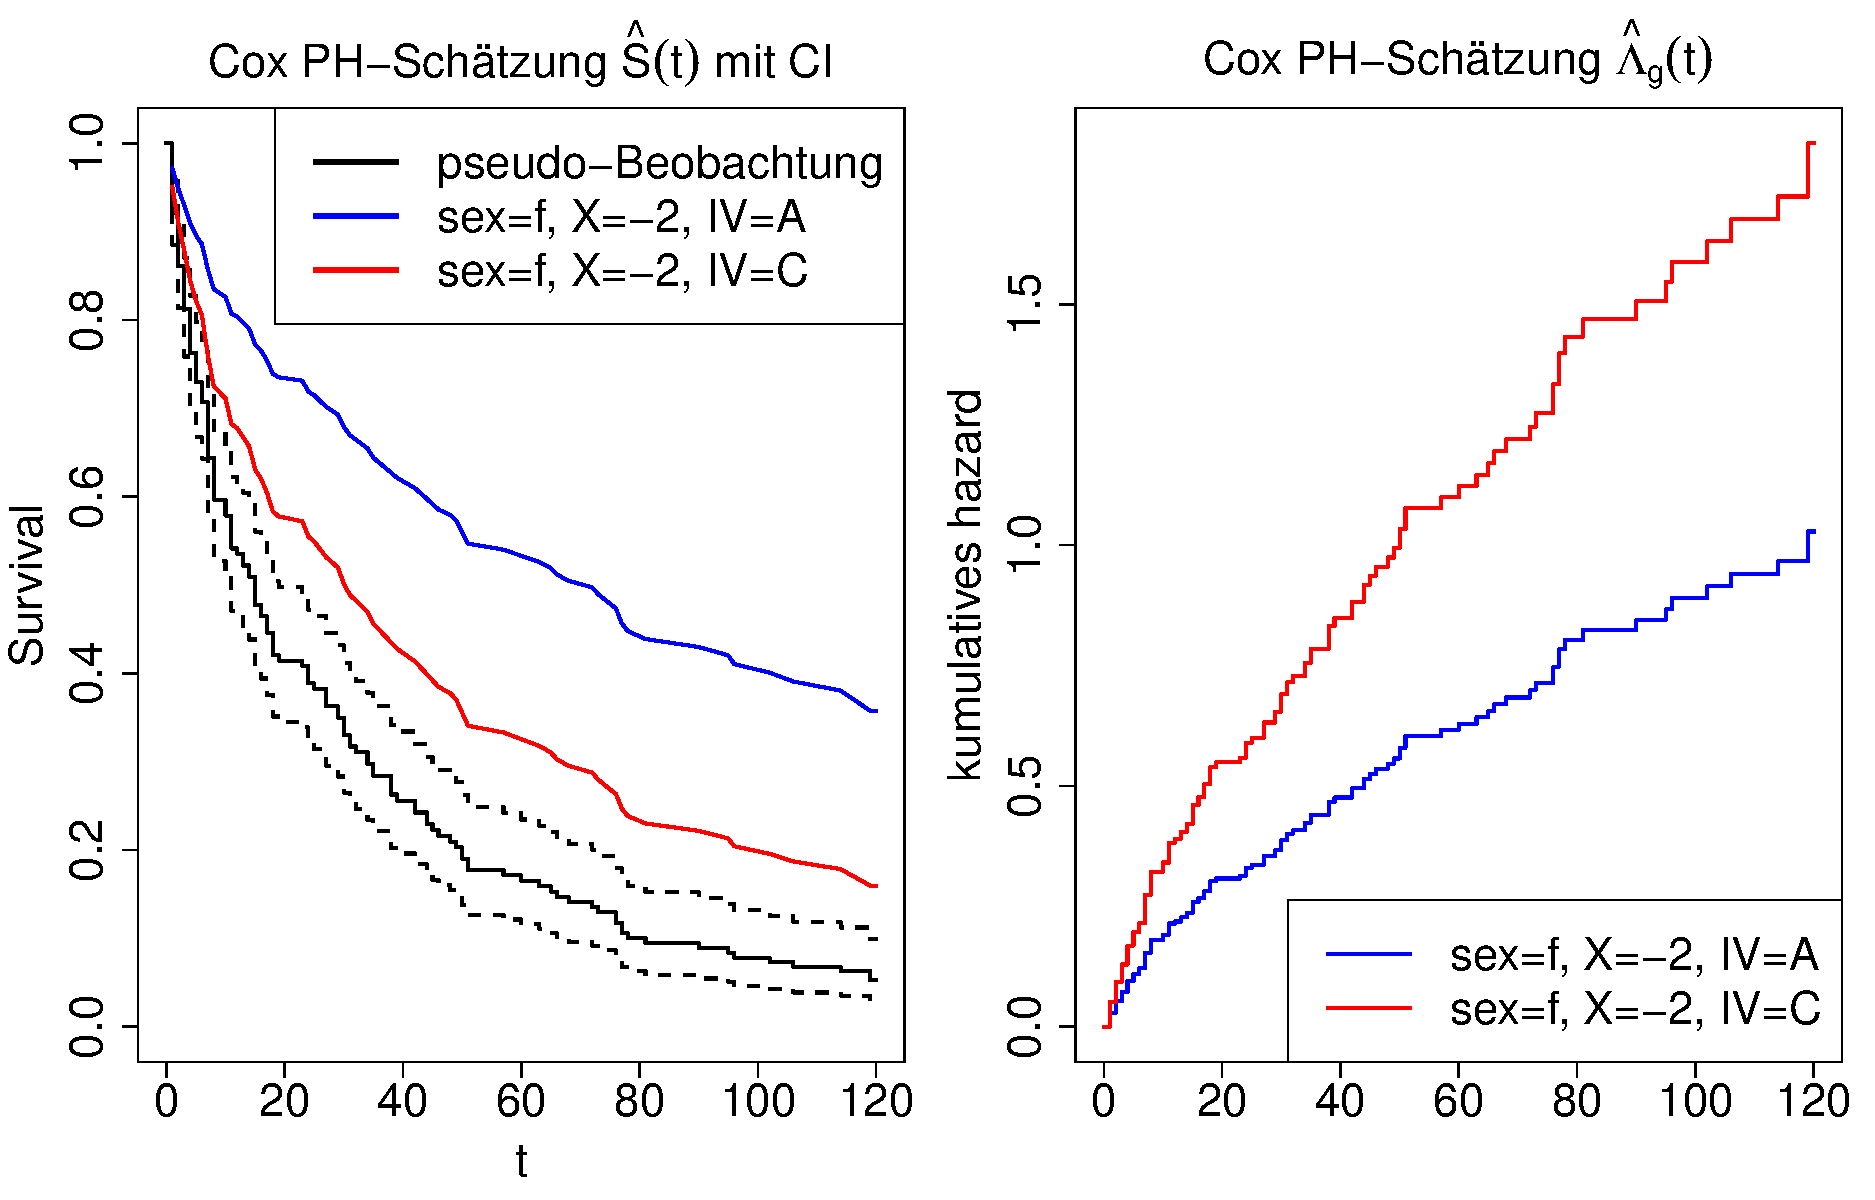
\includegraphics[width=12.5cm]{survivalCPH}
\vspace*{-1em}
\caption{Cox PH-Schätzungen: Survival-Funktion $\hat{S}_{\overline{\bm{x}}}(t)$ mit Konfidenzintervallen für ein pseudo-Beobachtungsobjekt mit mittleren Prädiktorwerten $\overline{\bm{x}}$ sowie kumulative Hazard-Funktion $\hat{\Lambda}_{g}(t)$ getrennt nach Gruppen $g$}
\label{fig:survivalCPH}
\end{figure}

Speziell für das geschätzte kumulative baseline hazard stellt das Paket\index[pack]{survival@\lstinline{survival}} \lstinline!survival! die Funktion\index[func]{basehaz()@\lstinline{basehaz()}} \lstinline!basehaz(<<coxph-Objekt>>)! als vereinfachte Variante von \lstinline!survfit()! zur Verfügung. Die Schätzung $\hat{\Lambda}_{\overline{\bm{x}}}(t)$ kann dabei mit dem Argument \lstinline!centered=TRUE! für ein pseudo-Beobachtungsobjekt berechnet werden, das für die vorliegende Stichprobe gemittelte Prädiktorwerte $\overline{\bm{x}}$ besitzt. Setzt man dagegen \lstinline!centered=FALSE!, bezieht sich das Ergebnis $\hat{\Lambda}_{0}(t)$ i.\,S.\ einer echten baseline bei Treatment-Kontrasten auf ein Beobachtungsobjekt in der Referenzgruppe jedes Faktors, für das alle Prädiktorwerte gleich $0$ sind. Das Ergebnis ist ein Datensatz mit den Variablen \lstinline!hazard! für $\hat{\Lambda}_{0}(t)$ und \lstinline!time! für $t$.

%%%%%%%%%%%%%%%%%%%%%%%%%%%%%%%%%%%%%%%%%%%%%%%%%%%%%%%%%%%%%%%%%%
%%%%%%%%%%%%%%%%%%%%%%%%%%%%%%%%%%%%%%%%%%%%%%%%%%%%%%%%%%%%%%%%%%
\subsection{Modelldiagnostik}
%%%%%%%%%%%%%%%%%%%%%%%%%%%%%%%%%%%%%%%%%%%%%%%%%%%%%%%%%%%%%%%%%%
%%%%%%%%%%%%%%%%%%%%%%%%%%%%%%%%%%%%%%%%%%%%%%%%%%%%%%%%%%%%%%%%%%

Um die Angemessenheit des Cox PH-Modells für die gegebenen Daten beurteilen zu können, sollten drei Aspekte der Modellanpassung geprüft werden: Die Annahme proportionaler hazards, das Vorhandensein besonders einflussreicher Beobachtungen sowie die Linearität von $\ln \lambda(t)$ bzgl.\ der kontinuierlichen Prädiktoren.

Aus der Annahme proportionaler hazards folgt, dass das logarithmierte kumulative hazard $\ln(-\ln(S(t)))$ linear mit $\ln t$ ist. Diese Voraussetzung lässt sich in einem Diagramm prüfen, das $\ln(-\ln(\hat{S}_{g}(t_{i})))$ gegen $\ln t_{i}$ aufträgt, wobei $\hat{S}_{g}(t_{i})$ die geschätzten Kaplan-Meier Survival-Funktionen der Überlebenszeit für die Stufen $g$ eines Faktors sind (Abb.\ \ref{fig:survivalDiagPHKM}). Dafür ist separat für jeden Prädiktor ein Kaplan-Meier Modell anzupassen und mit \lstinline!plot(<<KM-Modell>>, fun="cloglog")! darzustellen. Damit sich die PH-Annahme bzgl.\ kontinuierlicher Prädiktoren auf diese Weise prüfen lässt, müssen diese zunächst in Gruppen eingeteilt werden (Abschn.\ \ref{sec:cut}).

Die logarithmierten kumulativen hazards sollten im Diagramm linear mit $\ln t_{i}$ ansteigen und zudem parallel verlaufen. Im Spezialfall des Modells, das für $T$ eine Exponentialverteilung annimmt (Abschn.\ \ref{sec:survParam}), sollte die Steigung jeweils gleich $1$ sein. Ist die PH-Annahme offensichtlich für einen Prädiktor verletzt, besteht eine Strategie darin, bzgl.\ dieses Prädiktors zu stratifizieren -- bei kontinuierlichen Variablen nach Einteilung in geeignete Gruppen.
\begin{lstlisting}
> library(survival)             # für survfit(), cox.zph()
> dfSurv <- transform(dfSurv,   # teile X per Median-Split in 2 Gruppen
+                     Xcut=cut(X, breaks=c(-Inf, median(X), Inf)))

> KMiv   <- survfit(Surv(obsT, status) ~ IV,    # KM-Schätzungen für IV
+                   type="kaplan-meier", data=dfSurv)

> KMxcut <- survfit(Surv(obsT, status) ~ Xcut,  # KM-Schätzungen für X
+                   type="kaplan-meier", data=dfSurv)

# Diagramme ln(-ln(S(t))) gegen ln t
> plot(KMiv, fun="cloglog", main="cloglog-Plot für IV1",
+      xlab="ln t", ylab=expression(ln(-ln(hat(S)[g](t)))),
+      col=c("black", "blue", "red"), lty=1:3)

> legend(x="topleft", col=c("black", "blue", "red"), lwd=2,
+        lty=1:3, legend=LETTERS[1:3])

> plot(KMxcut, fun="cloglog", main="cloglog-Plot für Xcut",
+      xlab="ln t", ylab=expression(ln(-ln(hat(S)[g](t)))),
+      col=c("black", "blue"), lty=1:2)

> legend(x="topleft", col=c("black", "blue"), lwd=2,
+        legend=c("lo", "hi"), lty=1:2)
\end{lstlisting}

\begin{figure}[ht]
\centering
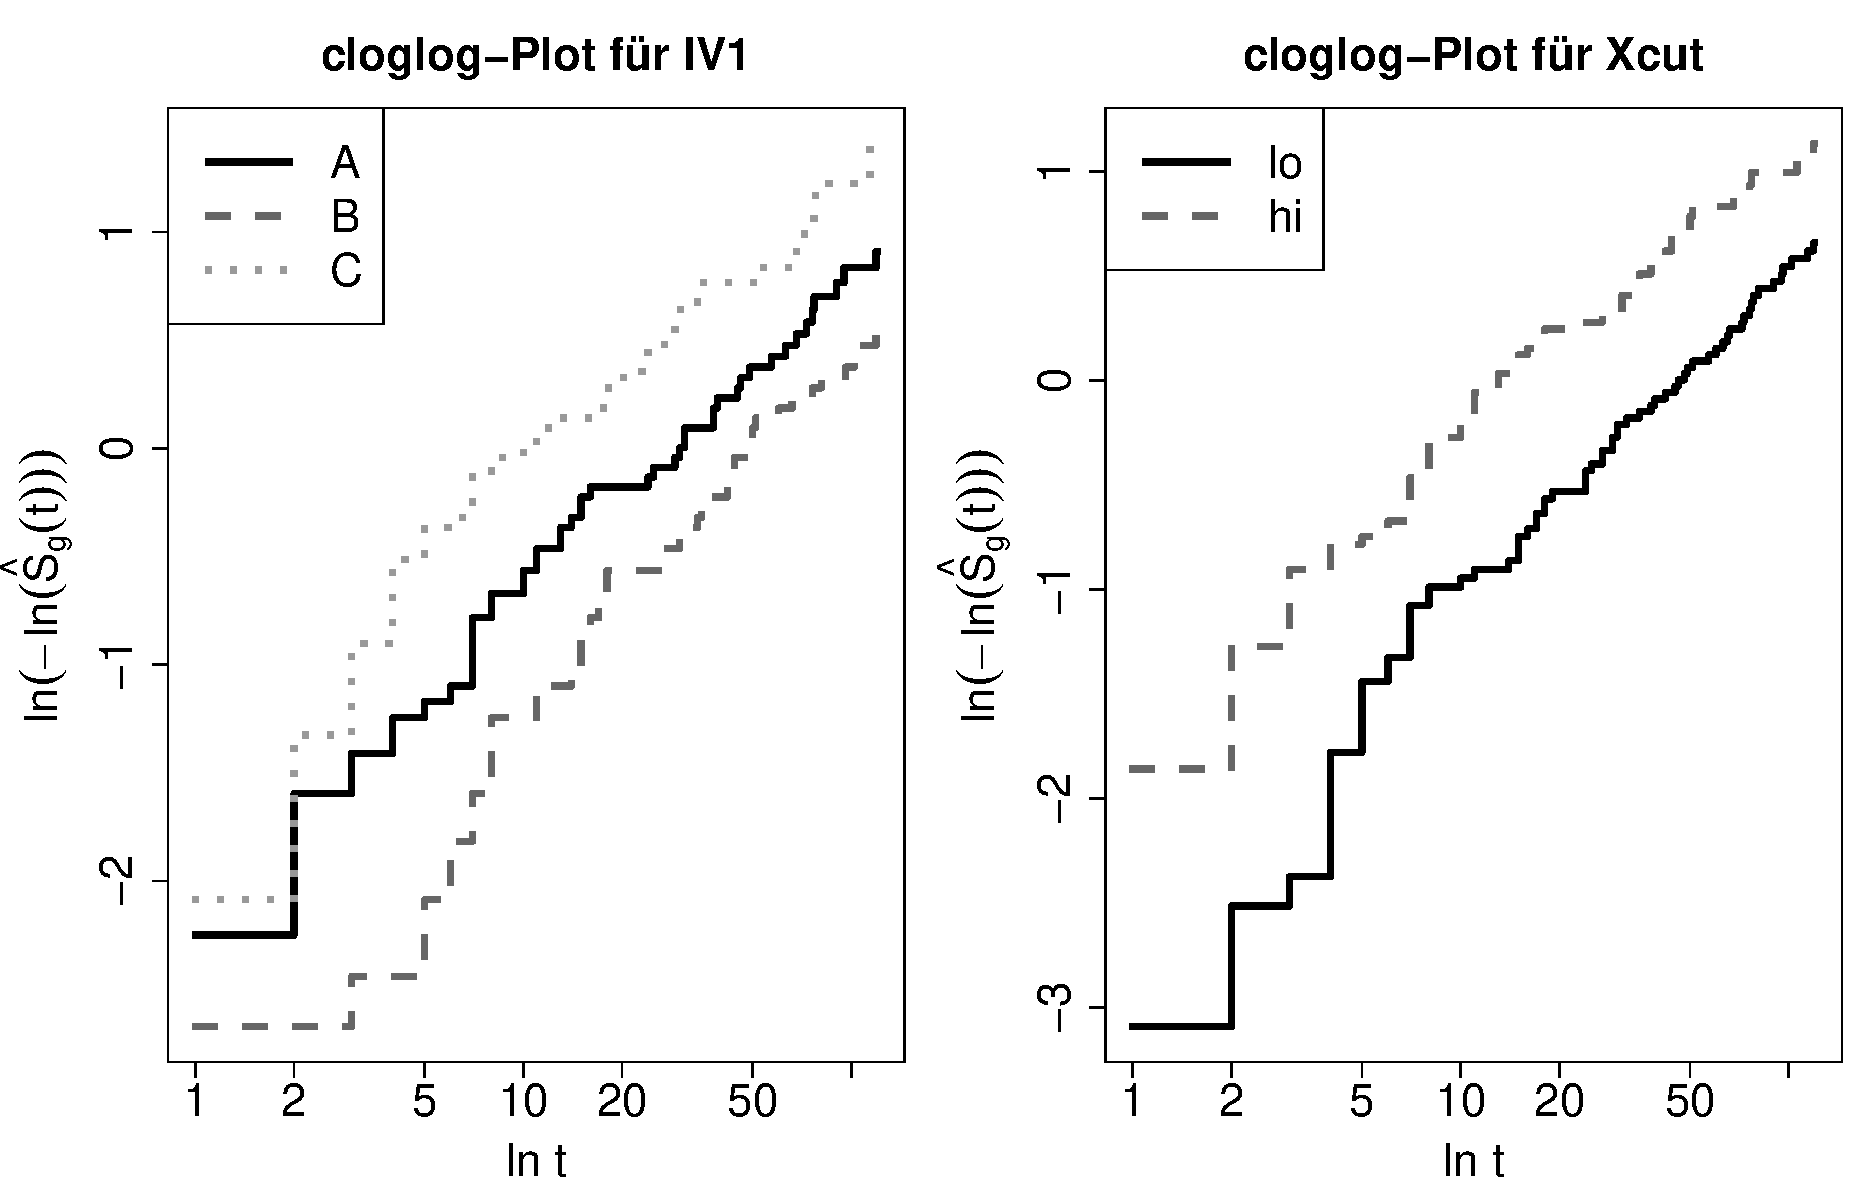
\includegraphics[width=12.5cm]{survivalDiagPHKM}
\vspace*{-1em}
\caption{Beurteilung der Annahme proportionaler hazards bzgl.\ jedes Prädiktors anhand der Linearität von $\ln(-\ln(\hat{S}_{g}(t_{i})))$ mit $\ln t_{i}$}
\label{fig:survivalDiagPHKM}
\end{figure}

Ähnlich wie in der Regressionsdiagnostik (Abschn.\ \ref{sec:regrDiag}) kann sich die Beurteilung der Voraussetzungen des Cox PH-Modells auch auf die Verteilung von Residuen stützen, insbesondere auf die Schönfeld- und Martingal-Residuen. Beide erhält man mit\index[func]{residuals()@\lstinline{residuals()}} \lstinline!residuals(<<coxph-Objekt>>, type="<<Typ>>")!, wobei \lstinline!type! auf \lstinline!"scaledsch"! bzw.\ auf \lstinline!"martingale"! zu setzen ist.

\lstinline!cox.zph(<<coxph-Objekt>>)!\index[func]{cox.zph()@\lstinline{cox.zph()}} berechnet ausgehend von der Korrelation der Schönfeld-Residuen mit einer Transformation der Überlebenszeit für jeden Prädiktor sowie für das Gesamtmodell einen $\chi^{2}$-Test der Nullhypothese, dass die Annahme proportionaler hazards stimmt.
\begin{lstlisting}
> (czph <- cox.zph(fitCPH))
           rho  chisq     p
X      -0.0959 1.5316 0.216
IVB     0.1001 1.6013 0.206
IVC     0.0216 0.0761 0.783
GLOBAL      NA 3.2264 0.358
\end{lstlisting}

Das von \lstinline!cox.zph()! ausgegebene Objekt lässt sich an \lstinline!plot()! übergeben, um die Schönfeld-Residuen für jeden Prädiktor gegen eine Transformation der Überlebenszeit darzustellen (Abb.\ \ref{fig:survivalDiagPH}). Die Diagramme enthalten zur Verdeutlichung des Verlaufs eine Spline-Interpolation (Abschn.\ \ref{sec:splines}) inkl.\ des zugehörigen Bereichs von $\pm 2$ Standardfehlern. Gibt es eine systematische Variation der Residuen in Abhängigkeit von der Überlebenszeit, ist das ein Hinweis darauf, dass die Annahme proportionaler hazards verletzt ist.
\begin{lstlisting}
> par(mfrow=c(2, 2))                            # Platz für 4 panels
> plot(czph)                                    # Residuen und splines
\end{lstlisting}

\begin{figure}[ht]
\centering
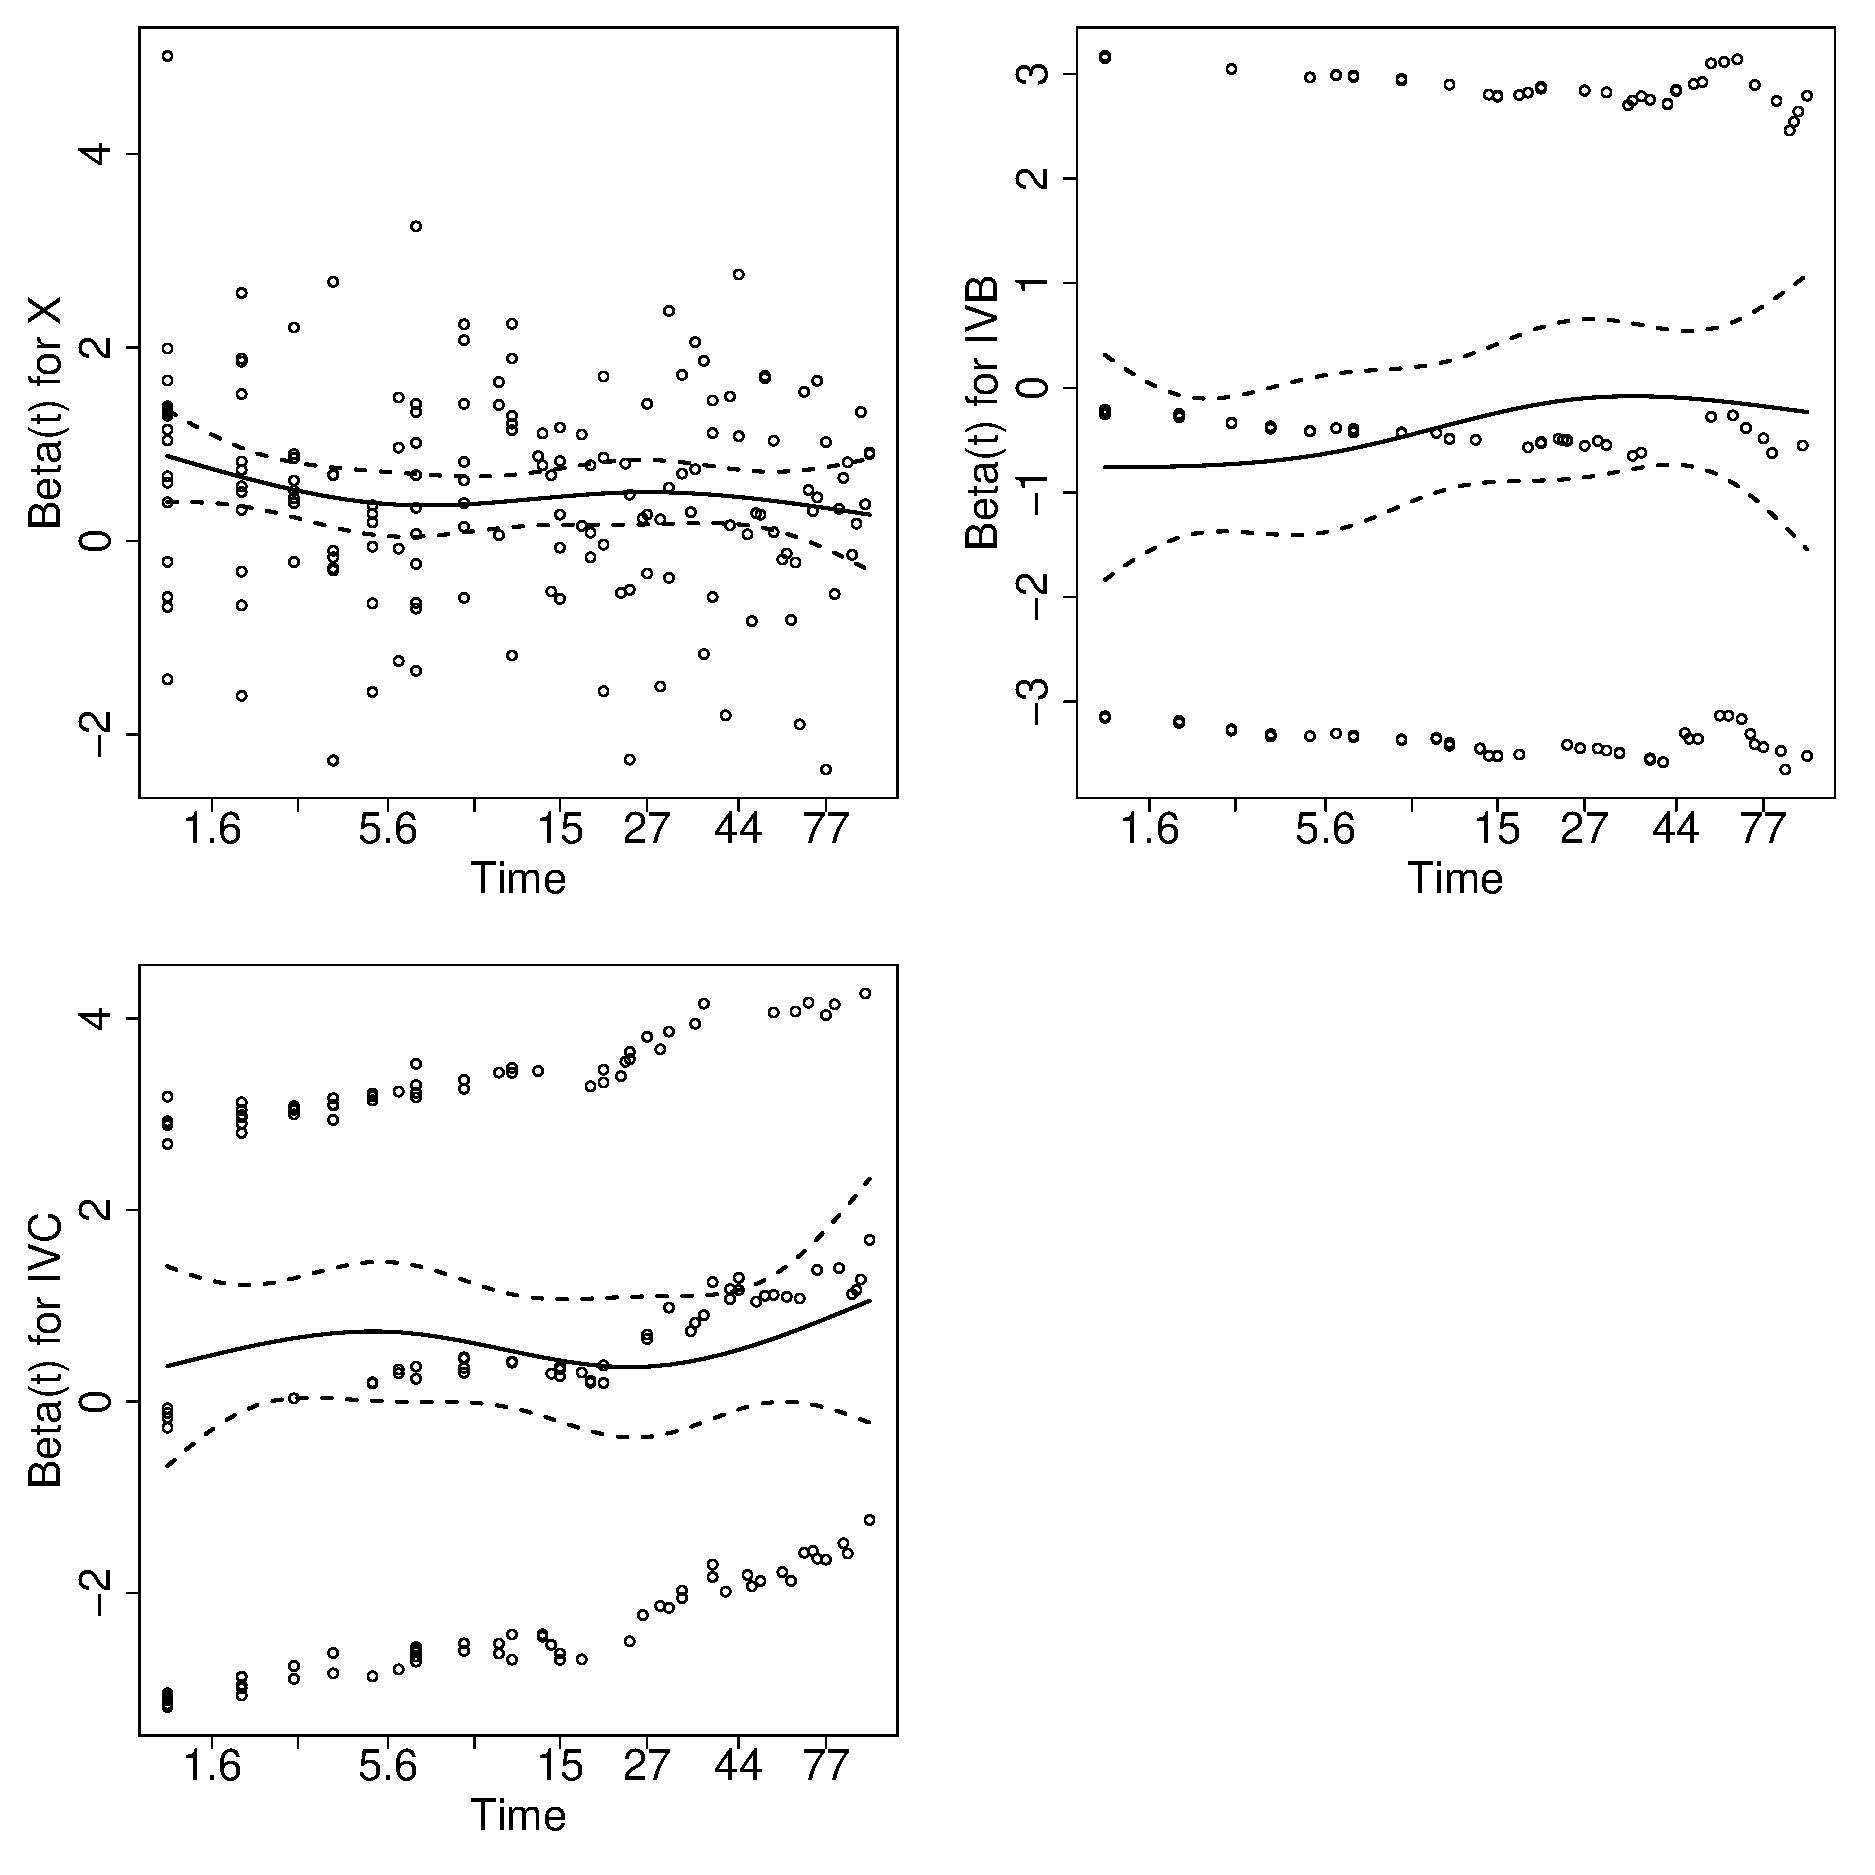
\includegraphics[width=12.5cm]{survivalDiagPH}
\vspace*{-1em}
\caption{Beurteilung der Annahme proportionaler hazards bzgl.\ jedes Prädiktors anhand skalierter Schönfeld-Residuen}
\label{fig:survivalDiagPH}
\end{figure}

Einflussreiche Beobachtungen können ähnlich wie in der linearen Regression über die von ihnen verursachten Änderungen in den geschätzten Parametern $\hat{\beta}_{j}$ diagnostiziert werden (Abschn.\ \ref{sec:regrInfluence}). Das standardisierte Maß DfBETAS erhält man für jede Beobachtung und jeden Prädiktor, indem man im Aufruf von \lstinline!residuals()! das Argument \lstinline!type="dfbetas"! wählt (Abb.\ \ref{fig:survivalDiagInflLin}).
\begin{lstlisting}
# Matrix der standardisierten Einflussgrößen DfBETAS
> dfbetas <- residuals(fitCPH, type="dfbetas")
> plot(dfbetas[ , 1], type="h", main="DfBETAS für X",
+      ylab="DfBETAS", lwd=2)

> plot(dfbetas[ , 2], type="h", main="DfBETAS für IV-B",
+      ylab="DfBETAS", lwd=2)

> plot(dfbetas[ , 3], type="h", main="DfBETAS für IV-C",
+      ylab="DfBETAS", lwd=2)
\end{lstlisting}

\begin{figure}[ht]
\centering
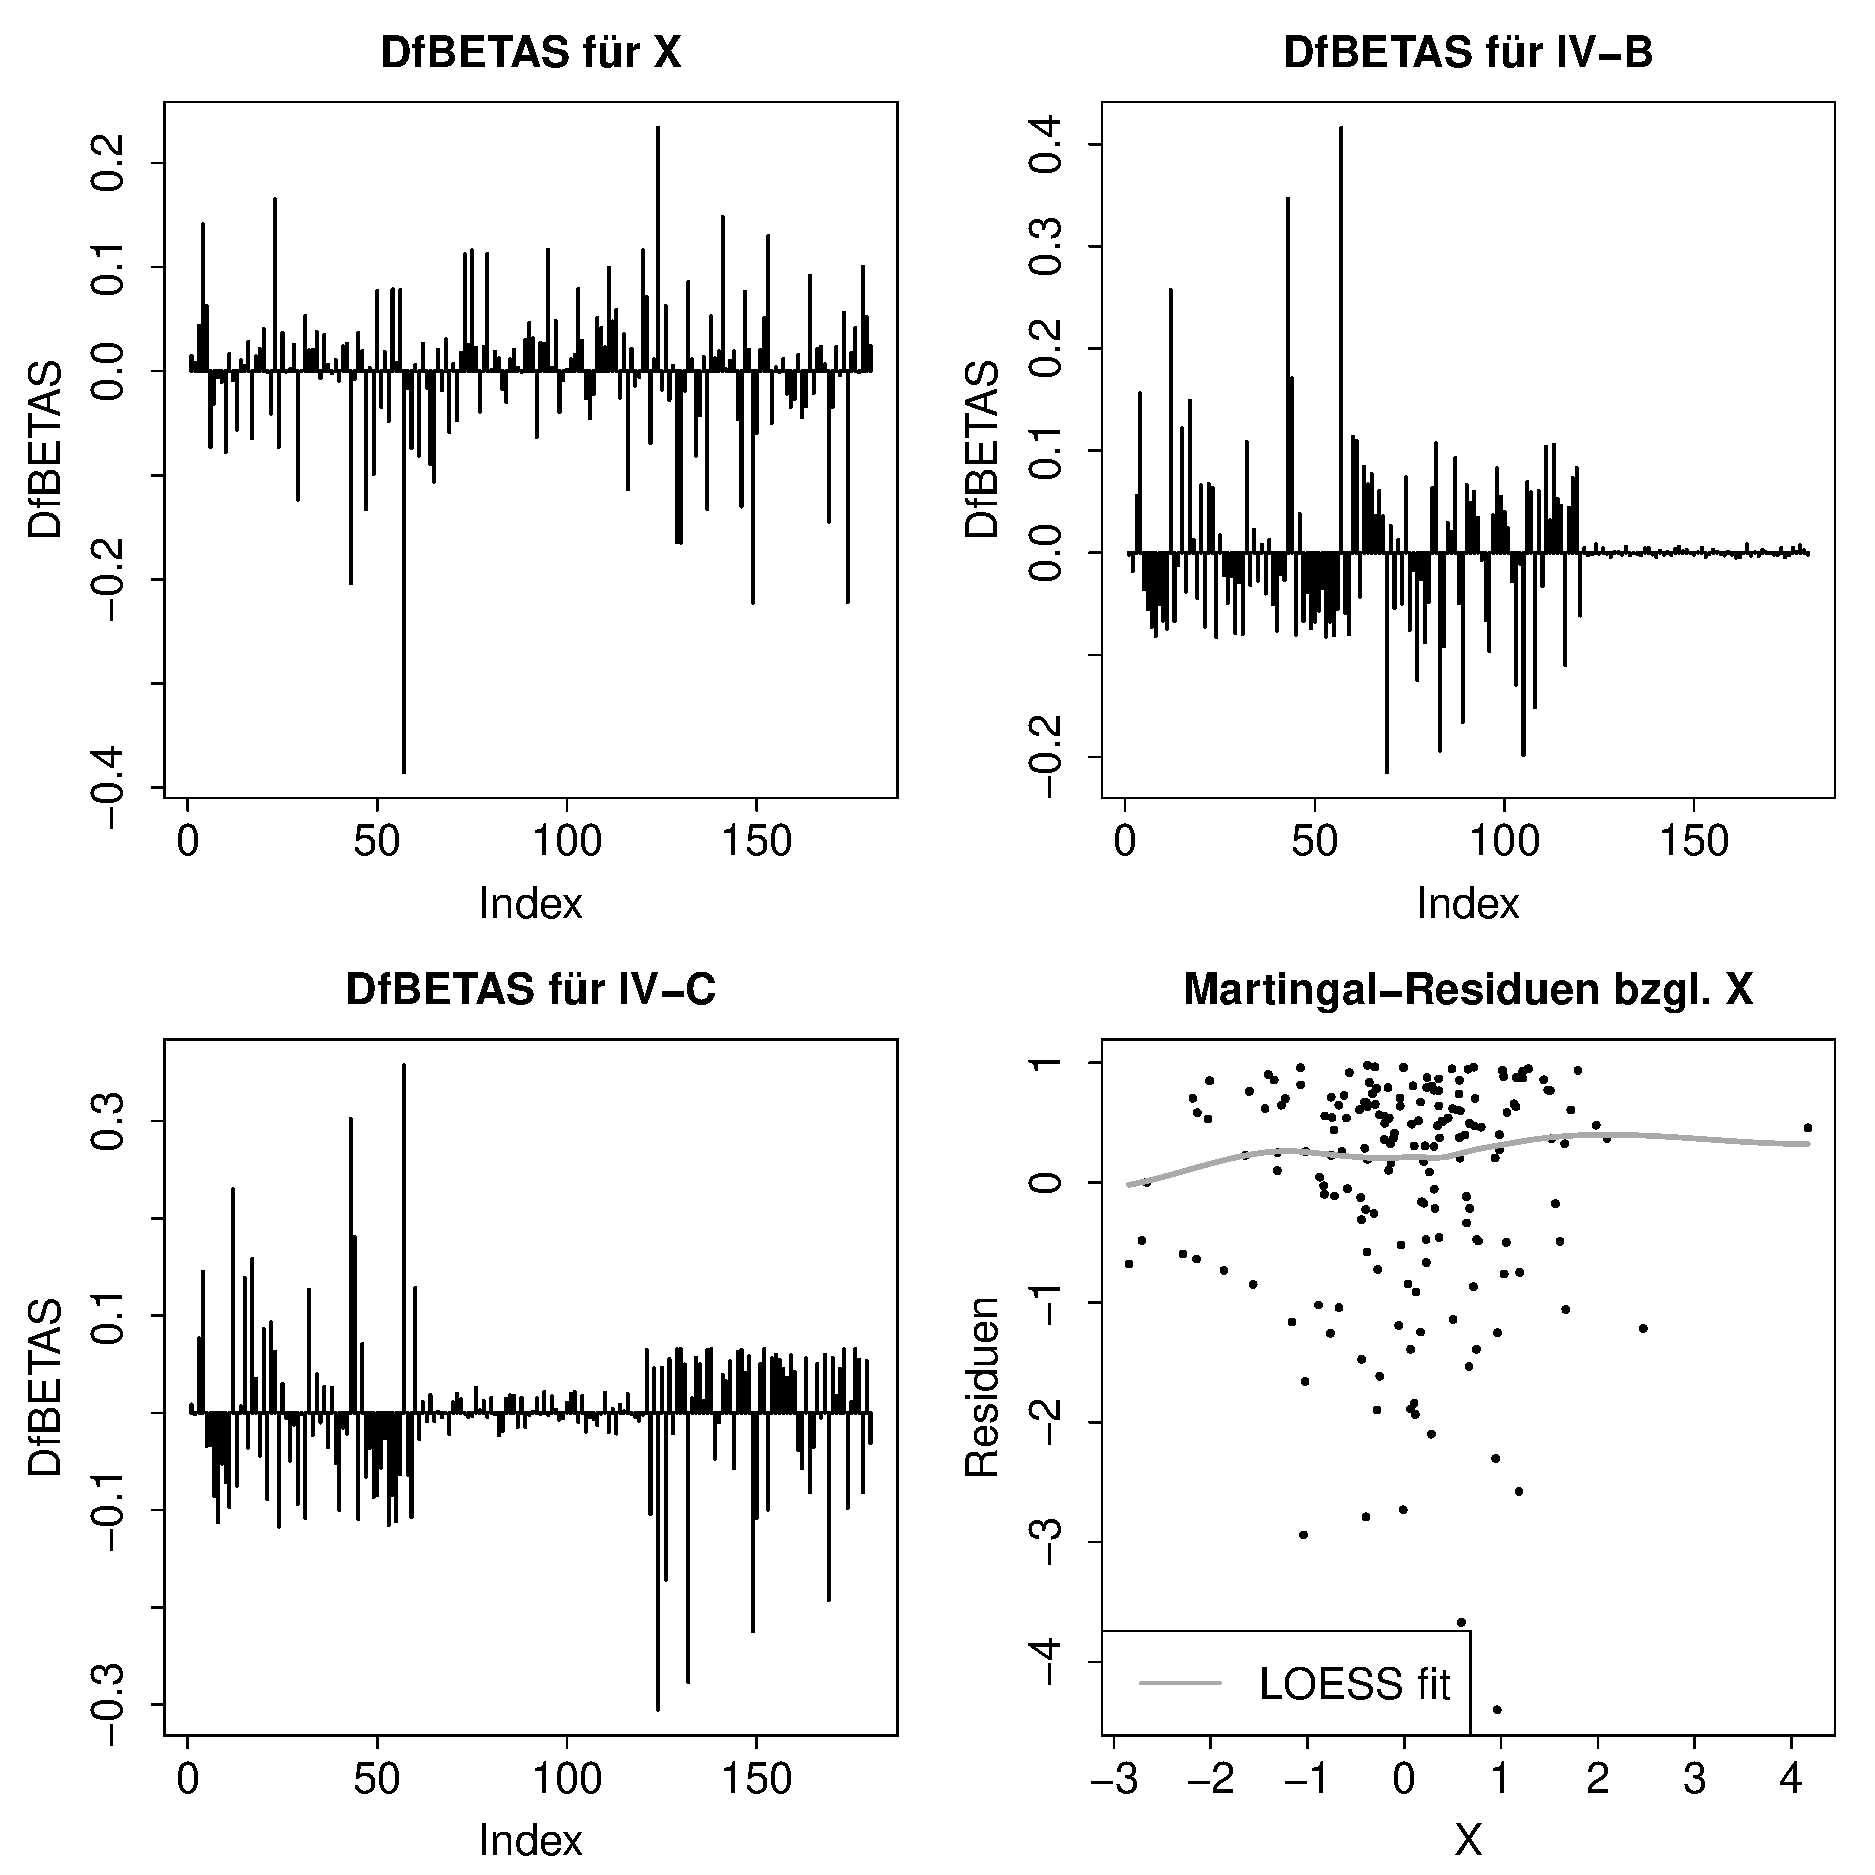
\includegraphics[width=12.5cm]{survivalDiagInflLin}
\vspace*{-0.5em}
\caption{Diagnostik einflussreicher Beobachtungen anhand der DfBETAS-Werte für jeden Prädiktor sowie Beurteilung der Linearität bzgl.\ des kontinuierlichen Prädiktors}
\label{fig:survivalDiagInflLin}
\end{figure}

Laut Modell sollte der Zusammenhang von $\ln \lambda(t)$ mit den Prädiktoren $X_{j}$ linear sein. Inwieweit die Daten mit dieser Annahme konsistent sind, lässt sich über den Verlauf der Martingal-Residuen in Abhängigkeit von den Werten der kontinuierlichen $X_{j}$ einschätzen (Abb.\ \ref{fig:survivalDiagInflLin}). Zur grafischen Beurteilung der Verteilung ist es dabei hilfreich, einen nonparametrichen LOESS-Glätter (Abschn.\ \ref{sec:loess}) einzuzeichnen, der horizontal verlaufen sollte.
\begin{lstlisting}
> resMart <- residuals(fitCPH, type="martingale")
> plot(dfSurv$X, resMart, main="Martingal-Residuen bzgl. X",
+      xlab="X", ylab="Residuen", pch=20)

# zeichne zusätzlich LOESS-Glätter ein
> lines(loess.smooth(dfSurv$X, resMart), lwd=2, col="blue")
> legend(x="bottomleft", col="blue", lwd=2, legend="LOESS fit")
\end{lstlisting}

%%%%%%%%%%%%%%%%%%%%%%%%%%%%%%%%%%%%%%%%%%%%%%%%%%%%%%%%%%%%%%%%%%
%%%%%%%%%%%%%%%%%%%%%%%%%%%%%%%%%%%%%%%%%%%%%%%%%%%%%%%%%%%%%%%%%%
\subsection{Vorhersage und Anwendung auf neue Daten}
\label{sec:survPredict}
%%%%%%%%%%%%%%%%%%%%%%%%%%%%%%%%%%%%%%%%%%%%%%%%%%%%%%%%%%%%%%%%%%
%%%%%%%%%%%%%%%%%%%%%%%%%%%%%%%%%%%%%%%%%%%%%%%%%%%%%%%%%%%%%%%%%%

Wie im GLM liefert\index[func]{predict()@\lstinline{predict()}} \lstinline!predict(<<coxph-Modell>>, type="<<Typ>>")! für jedes Beobachtungsobjekt $i$ Schätzungen verschiedener Kennwerte. Mit dem Argument \lstinline!type="risk"! erhält man die hazard ratios $\euler^{(\bm{x}_{i} - \overline{\bm{x}})' \hat{\bm{\beta}}}$ relativ zu einem pseudo-Beobachtungsobjekt, das als Prädiktorwerte den jeweiligen Mittelwert jedes Prädiktors aus der Stichprobe besitzt (kurz: $\overline{\bm{x}}$, s.\ Abschn.\ \ref{sec:CoxHat}). Für stratifizierte Modelle werden diese Mittelwerte dabei pro Schicht gebildet, es sei denn man setzt das Argument \lstinline!reference="sample"!. Für die Werte des linearen Prädiktors $\bm{X} \hat{\bm{\beta}}$ selbst ist \lstinline!type="lp"! zu verwenden.

Zusätzlich akzeptiert das Argument \lstinline!newdata! von \lstinline!predict()! einen Datensatz, der neue Daten für Variablen mit denselben Namen, und bei Faktoren auch denselben Stufen wie jene der ursprünglichen Prädiktoren enthält. Als Ergebnis erhält man die vorhergesagten hazard ratios für die neuen Prädiktorwerte (Abschn.\ \ref{sec:predict}).

%%%%%%%%%%%%%%%%%%%%%%%%%%%%%%%%%%%%%%%%%%%%%%%%%%%%%%%%%%%%%%%%%%
%%%%%%%%%%%%%%%%%%%%%%%%%%%%%%%%%%%%%%%%%%%%%%%%%%%%%%%%%%%%%%%%%%
\subsection{Erweiterungen des Cox PH-Modells}
\label{sec:coxExtend}
%%%%%%%%%%%%%%%%%%%%%%%%%%%%%%%%%%%%%%%%%%%%%%%%%%%%%%%%%%%%%%%%%%
%%%%%%%%%%%%%%%%%%%%%%%%%%%%%%%%%%%%%%%%%%%%%%%%%%%%%%%%%%%%%%%%%%

Das Cox PH-Modell lässt sich auf verschiedene Situationen erweitern:

\begin{itemize}
\item Zeitvariierende Kovariaten $X$ können über die Zählprozess-Darstellung von Daten (Abschn.\ \ref{sec:survTimeDep}) repräsentiert und etwa in Interaktionstermen $X \times t$ in die Modellformel von \lstinline!coxph()! aufgenommen werden. Dafür ist es notwendig, die Gesamt-Beobachtungsintervalle aller Personen mit \lstinline!survSplit()! an allen vorkommenden Ereignis-Zeitpunkten in Teilintervalle zu zerlegen. Details erläutert \lstinline!vignette("timedep", package="survival")!.
\item Pro Beobachtungsobjekt potentiell mehrfach auftretende Ereignisse lassen sich ebenfalls in Zählprozess-Darstellung speichern. In der Modellformel von \lstinline!coxph()! kann dann ein Vorhersageterm \lstinline!cluster(<<ID>>)! hinzugefügt werden, wobei der Faktor \lstinline!<<ID>>! codiert, von welchem Beobachtungsobjekt ein Intervall stammt. Dies bewirkt eine robuste Schätzung der Kovarianzmatrix der Parameterschätzer. Alternativ können wiederkehrende Ereignisse durch Stratifizierung analysiert werden, wobei die Beobachtungen mit jeweils dem ersten, zweiten, dritten, \ldots Ereignis ein Stratum bilden.
\item Penalisierte Cox-Modelle können mit der Funktion \lstinline!coxnet()!\index[func]{coxnet()@\lstinline{coxnet()}} aus dem Paket\index[pack]{glmnet@\lstinline{glmnet}} \lstinline!glmnet! (Abschn.\ \ref{sec:lmPen}) sowie mit dem Paket \index[pack]{coxphf@\lstinline{coxphf}} \lstinline!coxphf! \cite{Ploner2013} angepasst werden.
\item Für Hinweise zur Auswertung mit \emph{competing risks} \cite{Beyersmann2012} vgl.\ \lstinline!vignette("compete", package="survival")! und den Abschnitt \emph{Survival Analysis} der CRAN Task Views \cite{CRANtvSurvival}, letzteren auch für \emph{frailty} Modelle.
\end{itemize}

%%%%%%%%%%%%%%%%%%%%%%%%%%%%%%%%%%%%%%%%%%%%%%%%%%%%%%%%%%%%%%%%%%
%%%%%%%%%%%%%%%%%%%%%%%%%%%%%%%%%%%%%%%%%%%%%%%%%%%%%%%%%%%%%%%%%%
\section{Parametrische proportional hazards Modelle}
\label{sec:survParam}
%%%%%%%%%%%%%%%%%%%%%%%%%%%%%%%%%%%%%%%%%%%%%%%%%%%%%%%%%%%%%%%%%%
%%%%%%%%%%%%%%%%%%%%%%%%%%%%%%%%%%%%%%%%%%%%%%%%%%%%%%%%%%%%%%%%%%

\index{Survival-Analyse!parametrische Modelle}
Bei spezifischen Vorstellungen über die Verteilung der Überlebenszeit $T$ kommen auch parametrische Regressionsmodelle in Betracht, die sich unter Beibehaltung der Annahme proportionaler hazards als Spezialfälle des Cox PH-Modells ergeben (Abschn.\ \ref{sec:survCPH}). Für exponential- oder Weibull-verteilte Überlebenszeiten gibt es dabei zwei äquivalente Möglichkeiten, das lineare Regressionsmodell zu formulieren: Zum einen wie im Cox PH-Modell für das logarithmierte hazard, zum anderen für die logarithmierte Überlebenszeit. Bei der zweiten Darstellung spricht man von einem \emph{accelerated failure time} Modell (AFT).  Da in parametrischen Modellen das hazard voll spezifiziert ist, lassen sie sich anders als Cox PH-Modelle auch zur Vorhersage jenseits des letzten beobachteten Ereignisses nutzen.

%%%%%%%%%%%%%%%%%%%%%%%%%%%%%%%%%%%%%%%%%%%%%%%%%%%%%%%%%%%%%%%%%%
%%%%%%%%%%%%%%%%%%%%%%%%%%%%%%%%%%%%%%%%%%%%%%%%%%%%%%%%%%%%%%%%%%
\subsection{Darstellung über die Hazard-Funktion}
%%%%%%%%%%%%%%%%%%%%%%%%%%%%%%%%%%%%%%%%%%%%%%%%%%%%%%%%%%%%%%%%%%
%%%%%%%%%%%%%%%%%%%%%%%%%%%%%%%%%%%%%%%%%%%%%%%%%%%%%%%%%%%%%%%%%%

Spezialfälle des Cox PH-Modells ergeben sich, wenn für das baseline hazard $\lambda_{0}(t)$ eine Verteilung angenommen wird, die mit einer Exponential- oder Weibull-Verteilung von $T$ korrespondiert. Die logarithmierte Ereignisrate soll wie im Cox PH-Modell linear von den Prädiktoren $X_{j}$ abhängen. Das baseline hazard $\lambda_{0}(t)$ ist dabei der Verlauf der Ereignisrate für ein Beobachtungsobjekt, für das alle $X_{j}$ gleich $0$ bzw.\ alle Faktoren gleich der Referenzkategorie sind (bei Treatment-Kontrasten). Die exponenzierten Parameter $\euler^{\beta_{j}}$ geben wie im Cox PH-Modell den Änderungsfaktor für die Ereignisrate (also das hazard ratio) an, wenn ein Prädiktor um $1$ wächst.

Bei Annahme einer Exponentialverteilung von $T$ mit Erwartungswert $E(T) = b > 0$ und Varianz $b^{2}$ ergibt sich die Dichtefunktion $f(t) = \lambda(t) \, S(t)$ aus der konstanten Hazard-Funktion $\lambda(t) = \lambda = \frac{1}{b}$ und der Survival-Funktion $S(t) = \euler^{-\frac{t}{b}}$. Die kumulative Hazard-Funktion ist $\Lambda(t) = \frac{t}{b}$. Oft wird die Exponentialverteilung auch mit der Grundrate $\lambda$ als $f(t) = \lambda \, \euler^{-\lambda t}$ bzw.\ $S(t) = \euler^{-\lambda t}$ und $\Lambda(t) = \lambda t$ formuliert. In \lstinline!rexp()! ist mit dem Argument \lstinline!rate! $\lambda$ gemeint. Durch den Einfluss der $X_{j}$ ergibt sich dann als neue Grundrate $\lambda' = \lambda \, \euler^{\bm{X} \bm{\beta}}$. Insgesamt resultieren aus der Spezialisierung des Cox PH-Modells folgende Modellvorstellungen, wobei die Abkürzung $\bm{X} \bm{\beta}$ keinen absoluten Term $\beta_{0}$ einschließt:
\begin{equation*}
\begin{array}{rclcl}
\lambda(t)     &=& \frac{1}{b} \, \euler^{\bm{X} \bm{\beta}} &=& \lambda \, \euler^{\bm{X} \bm{\beta}}\\
\ln \lambda(t) &=& -\ln b + \bm{X} \bm{\beta} &=& \ln \lambda + \bm{X} \bm{\beta}\\
S(t)           &=& \exp\left(-\frac{t}{b} \, \euler^{\bm{X} \bm{\beta}}\right) &=& \exp\left(-\lambda \, t \, \euler^{\bm{X} \bm{\beta}}\right)\\
\Lambda(t)     &=& \frac{t}{b} \, \euler^{\bm{X} \bm{\beta}} &=& \lambda \, t \, \euler^{\bm{X} \bm{\beta}}
\end{array}
\end{equation*}

Die Dichtefunktion einer Weibull-Verteilung kann unterschiedlich formuliert werden. \lstinline!dweibull()! verwendet den Formparameter $a > 0$ für das Argument \lstinline!shape! und den Skalierungsparameter $b > 0$ für \lstinline!scale!. Für $a > 1$ steigt das hazard mit $t$, für $a < 1$ sinkt es, und für $a = 1$ ist es konstant. Die Exponentialverteilung ist also ein Spezialfall der Weibull-Verteilung für $a = 1$. $b$ ist die \emph{charakteristische Lebensdauer}, nach der $1-\frac{1}{\euler} \approx 63.2\%$ der Ereignisse aufgetreten sind ($S(b) = \frac{1}{\euler}$). Die Dichtefunktion $f(t) = \lambda(t) \, S(t)$ ergibt sich mit dieser Wahl aus der Hazard-Funktion $\lambda(t) = \frac{a}{b} \left(\frac{t}{b}\right)^{a-1}$ und der Survival-Funktion $S(t) = \exp(-(\frac{t}{b})^{a})$. Die kumulative Hazard-Funktion ist $\Lambda(t) = (\frac{t}{b})^{a}$ mit der Umkehrfunktion $\Lambda^{-1}(t) = (b \, t)^{\frac{1}{a}}$. Der Erwartungswert ist $E(T) = b \, \Gamma(1 + \frac{1}{a})$.

Analog zur Exponentialverteilung lässt sich die Weibull-Verteilung auch mit $\lambda = \frac{1}{b^{a}}$ formulieren, so dass $\lambda(t) = \lambda \, a \, t^{a-1}$, $S(t) = \exp(-\lambda \, t^{a})$ und $\Lambda(t) = \lambda \, t^{a}$ gilt. Durch den Einfluss der $X_{j}$ ergibt sich dann $\lambda' = \lambda \, \euler^{\bm{X} \bm{\beta}}$. Insgesamt impliziert das Weibull-Modell folgende Zusammenhänge:
\begin{equation*}
\begin{array}{rclcl}
\lambda(t)     &=& \frac{a}{b} \left(\frac{t}{b}\right)^{a-1} \, \euler^{\bm{X} \bm{\beta}} &=& \lambda \, a \, t^{a-1} \, \euler^{\bm{X} \bm{\beta}}\\
\ln \lambda(t) &=& \ln \left(\frac{a}{b} \left(\frac{t}{b}\right)^{a-1}\right) + \bm{X} \bm{\beta} &=& \ln \lambda + \ln a + (a-1) \, \ln t + \bm{X} \bm{\beta}\\
S(t)           &=& \exp\left(-(\frac{t}{b})^{a} \, \euler^{\bm{X} \bm{\beta}}\right) &=& \exp\left(-\lambda \, t^{a} \, \euler^{\bm{X} \bm{\beta}}\right)\\
\Lambda(t)     &=& (\frac{t}{b})^{a} \, \euler^{\bm{X} \bm{\beta}} &=& \lambda \, t^{a} \, \euler^{\bm{X} \bm{\beta}}
\end{array}
\end{equation*}

%%%%%%%%%%%%%%%%%%%%%%%%%%%%%%%%%%%%%%%%%%%%%%%%%%%%%%%%%%%%%%%%%%
%%%%%%%%%%%%%%%%%%%%%%%%%%%%%%%%%%%%%%%%%%%%%%%%%%%%%%%%%%%%%%%%%%
\subsection{Darstellung als accelerated failure time Modell}
%%%%%%%%%%%%%%%%%%%%%%%%%%%%%%%%%%%%%%%%%%%%%%%%%%%%%%%%%%%%%%%%%%
%%%%%%%%%%%%%%%%%%%%%%%%%%%%%%%%%%%%%%%%%%%%%%%%%%%%%%%%%%%%%%%%%%

Das betrachtete Exponential- und Weibull-Modell lässt sich äquivalent auch jeweils als lineares Modell der logarithmierten Überlebenszeit formulieren (accelerated failure time Modell, AFT).
\begin{equation*}
\begin{array}{rclcl}
\ln T &=& \bm{X} \bm{\gamma} + \bm{z} &=& \bm{\mu} + \sigma \bm{\epsilon}\\
\end{array}
\end{equation*}

Dabei ist $\epsilon$ ein Fehlerterm, der im Weibull-Modell einer Typ-I (Gumbel) Extremwertverteilung folgt und durch $\sigma = \frac{1}{a}$ skaliert wird. Sind $t_{i}$ zufällige Überlebenszeiten aus einer Weibull-Verteilung, sind damit $\ln t_{i}$ zufällige Beobachtungen einer Extremwertverteilung mit Erwartungswert $\mu = \ln b$. Mit $a = 1$ ergibt sich als Spezialfall das Exponential-Modell.

Ein Parameter $\gamma_{j}$ ist im AFT-Modell das über $t$ konstante Verhältnis zweier Quantile von $S(t)$, wenn sich der Prädiktor $X_{j}$ um eine Einheit erhöht. Ein exponenzierter Parameter $\euler^{\gamma_{j}}$ gibt analog den Änderungsfaktor für die Überlebenszeit bei einer Änderung von $X_{j}$ um eine Einheit an. Zwischen dem Parameter $\beta_{j}$ in der Darstellung als PH-Modell und dem Parameter $\gamma_{j}$ in der Formulierung als AFT-Modell besteht für Weibull-verteilte Überlebenszeiten die Beziehung $\beta_{j} = -\frac{\gamma_{j}}{a}$, für den Spezialfall exponentialverteilter Überlebenszeiten also $\beta_{j} = -\gamma_{j}$.

%%%%%%%%%%%%%%%%%%%%%%%%%%%%%%%%%%%%%%%%%%%%%%%%%%%%%%%%%%%%%%%%%%
%%%%%%%%%%%%%%%%%%%%%%%%%%%%%%%%%%%%%%%%%%%%%%%%%%%%%%%%%%%%%%%%%%
\subsection{Anpassung und Modelltests}
%%%%%%%%%%%%%%%%%%%%%%%%%%%%%%%%%%%%%%%%%%%%%%%%%%%%%%%%%%%%%%%%%%
%%%%%%%%%%%%%%%%%%%%%%%%%%%%%%%%%%%%%%%%%%%%%%%%%%%%%%%%%%%%%%%%%%

AFT-Modelle können mit\index[func]{survreg()@\lstinline{survreg()}} \lstinline!survreg()! aus dem Paket\index[pack]{survival@\lstinline{survival}} \lstinline!survival! angepasst werden.
\begin{lstlisting}
survreg(<<Modellformel>>, dist="<<Verteilung>>", data=<<Datensatz>>)
\end{lstlisting}

Als erstes Argument ist eine Modellformel zu übergeben, deren linke Seite ein mit \lstinline!Surv()! erstelltes Objekt ist (Abschn.\ \ref{sec:survData}). Dabei ist sicherzustellen, dass alle Ereignis-Zeitpunkte $t_{i} > 0$ sind und nicht (etwa durch Rundung) Nullen enthalten. Die rechte Seite der Modellformel kann neben -- zeitlich konstanten -- kontinuierlichen Prädiktoren und Faktoren als besonderen Vorhersageterm \lstinline!strata(<<Faktor>>)! umfassen. Dieser sorgt dafür, dass ein stratifiziertes Modell angepasst wird, das eine separate Baseline-Hazard-Funktion $\lambda_{0_{g}}(t)$ für jede Stufe $g$ des Faktors beinhaltet. Stammen die in der Modellformel verwendeten Variablen aus einem Datensatz, ist dieser unter \lstinline!data! zu nennen. Das Argument \lstinline!dist! bestimmt die für $T$ angenommene Verteilung -- mögliche Werte sind unter Annahme proportionaler hazards \lstinline!"weibull"! oder \lstinline!"exponential"!.\footnote{Verzichtet man auf die Annahme proportionaler hazards, kommen auch weitere Verteilungen für $T$ in Betracht, über die \lstinline!?survreg! Auskunft gibt.}

Die Modelle sollen hier für die in Abschn.\ \ref{sec:survTimeInd} simulierten Daten mit zeitlich konstanten Prädiktoren und höchstens einmal auftretenden Ereignissen angepasst werden.
\begin{lstlisting}
> library(survival)                       # für survreg()
> fitWeib <- survreg(Surv(obsT, status) ~ X + IV, dist="weibull",
+                    data=dfSurv)
\end{lstlisting}

Wald-Tests der Parameter sowie einen Likelihood-Quotienten-Test des Gesamtmodells erhält man mit \lstinline!summary(<<survreg-Objekt>>)!.
\begin{lstlisting}
> summary(fitWeib)                        # Parameter- und Modelltests
             Value Std. Error     z        p
(Intercept)  3.423     0.1703 20.10 7.45e-90
X           -0.632     0.1024 -6.17 6.65e-10
IVB          0.504     0.2449  2.06 3.94e-02
IVC         -0.778     0.2327 -3.34 8.29e-04
Log(scale)   0.216     0.0608  3.56 3.73e-04

Scale=1.24

Weibull distribution
Loglik(model)= -695.9   Loglik(intercept only)= -726.9
        Chisq= 62.03 on 3 degrees of freedom, p= 2.2e-13
Number of Newton-Raphson Iterations: 5
n=180
\end{lstlisting}

Die Ausgabe ist weitgehend analog zu jener von \lstinline!summary(<<coxph-Objekt>>)! (Abschn.\ \ref{sec:survCPH}), wobei in der Spalte \lstinline!Value! die geschätzten AFT-Parameter $\hat{\gamma}_{j} = - \hat{\beta}_{j} \cdot \hat{a}$ genannt werden.\footnote{Für die $\hat{\beta}_{j}$ ergibt sich $0.51$ (\lstinline!X!), $-0.41$ (\lstinline!IVB!) und $0.63$ (\lstinline!IVC!) -- also Schätzungen, die hier denen des Cox PH-Modells sehr ähnlich sind (s.\ S.\ \pageref{sec:survCPHres}).} Die Schätzung $\hat{a}$ des Formparameters der Weibull-Verteilung ist unter \lstinline!Scale! aufgeführt. Der zugehörige Wald-Test mit der $\text{H}_{0}$: $\ln a = 0$ steht in der Zeile \lstinline!Log(scale)!. Eine Alternative hierzu ist der Likelihood-Quotienten-Test des eingeschränkten Modells \lstinline!<<fitR>>! mit Exponentialverteilung ($a = 1$, also $\ln a = 0$) gegen das umfassendere Modell \lstinline!<<fitU>>! mit Weibull-Verteilung mittels \lstinline!anova(<<fitR>>, <<fitU>>)! (Abschn.\ \ref{sec:regrLogTest}).
\begin{lstlisting}
# eingeschränktes Modell mit a=1 -> Exponentialverteilung
> fitExp <- survreg(Surv(obsT, status) ~ X + IV, dist="exponential",
+                   data=dfSurv)

> anova(fitExp, fitWeib)                  # LQ-Modelltest
   Terms Resid. Df    -2*LL Test Df Deviance     Pr(>Chi)
1 X + IV       176 1405.946      NA       NA           NA
2 X + IV       175 1391.839    =  1 14.10752 0.0001726517
\end{lstlisting}

Da der hier im Modell berücksichtigte Faktor \lstinline!IV! mit mehreren Parametern $\gamma_{j}$ assoziiert ist, muss seine Signifikanz insgesamt über einen Modellvergleich getestet werden. Dazu dient wie beim Vergleich der Modelle mit Exponential- und Weibull-Verteilung ein Likelihood-Quotienten-Test zweier hierarchischer Modelle.
\begin{lstlisting}
# eingeschränktes Modell ohne Faktor IV
> fitR <- survreg(Surv(obsT, status) ~ X, dist="weibull", data=dfSurv)
> anova(fitR, fitWeib)                    # LQ-Modelltest für Faktor IV
   Terms Resid. Df    -2*LL Test Df Deviance     Pr(>Chi)
1      X       177 1418.773
2 X + IV       175 1391.839  +IV  2 26.93433 1.416721e-06
\end{lstlisting}

%%%%%%%%%%%%%%%%%%%%%%%%%%%%%%%%%%%%%%%%%%%%%%%%%%%%%%%%%%%%%%%%%%
%%%%%%%%%%%%%%%%%%%%%%%%%%%%%%%%%%%%%%%%%%%%%%%%%%%%%%%%%%%%%%%%%%
\subsection{Survival-Funktion schätzen}
%%%%%%%%%%%%%%%%%%%%%%%%%%%%%%%%%%%%%%%%%%%%%%%%%%%%%%%%%%%%%%%%%%
%%%%%%%%%%%%%%%%%%%%%%%%%%%%%%%%%%%%%%%%%%%%%%%%%%%%%%%%%%%%%%%%%%

Die geschätzte Verteilungsfunktion $\hat{F}(t)$ für ein mit \lstinline!survreg()! angepasstes Modell ermittelt \lstinline!predict()! (Abschn.\ \ref{sec:predict}). Die meist stattdessen betrachtete geschätzte Survival-Funktion ergibt sich daraus als $\hat{S}(t) = 1-\hat{F}(t)$.
\begin{lstlisting}
predict(<<survreg-Objekt>>, newdata=<<Datensatz>>, type="quantile",
        p=<<Quantile>>, se=TRUE)
\end{lstlisting}

Als erstes Argument ist ein \lstinline!survreg!-Objekt zu übergeben. Das Argument \lstinline!newdata! erwartet einen Datensatz, der neue Daten für Variablen mit denselben Namen, und bei Faktoren auch denselben Stufen wie jene der ursprünglichen Prädiktoren im \lstinline!survreg!-Objekt enthält. Mit dem Argument \lstinline!type="quantile"! liefert \lstinline!predict()! für jede Zeile in \lstinline!newdata! für das Quantil $p \in (0, 1)$ den Wert $\hat{F}^{-1}(p)$. Dies ist die Überlebenszeit $t_{p}$, für die bei den in \lstinline!newdata! gegebenen Gruppenzugehörigkeiten und Prädiktorwerten $\hat{F}(t_{p}) = p$ gilt. Dafür ist an \lstinline!p! ein Vektor mit Quantilen zu übergeben, deren zugehörige Werte von $\hat{F}(t)$ gewünscht werden. Den geschätzten Median der Überlebenszeit erfährt man etwa mit \lstinline!p=0.5!, während für einen durchgehenden Funktionsgraphen von $\hat{F}(t)$ bzw. $\hat{S}(t)$ eine fein abgestufte Sequenz im Bereich $(0, 1)$ angegeben werden muss. Setzt man \lstinline!se=TRUE!, erhält man zusätzlich noch die geschätzte Streuung von $\hat{F}(t)$.

Mit \lstinline!se=TRUE! ist das zurückgegebene Objekt eine Liste mit den Werten von $\hat{F}^{-1}(p)$ in der Komponente \lstinline!fit! und den geschätzten Streuungen in der Komponente \lstinline!se.fit!. Umfasst \lstinline!newdata! mehrere Zeilen, sind \lstinline!fit! und \lstinline!se.fit! Matrizen mit einer Zeile pro Beobachtungsobjekt und einer Spalte pro Quantil.\footnote{Abschnitt \ref{sec:CoxHat} demonstriert die analoge Verwendung von \lstinline!newdata! in \lstinline!survfit()!.}
\begin{lstlisting}
# Datensatz: 2 Männer mit Prädiktor X=0 in Gruppe A bzw. in C
> dfNew <- data.frame(sex=factor(c("m","m"), levels=levels(dfSurv$sex)),
+                       X=c(0, 0),
+                      IV=factor(c("A", "C"), levels=levels(dfSurv$IV)))

# geschätzte Werte von F^(-1)
> percs <- (1:99)/100                         # Perzentile = Quantile
> FWeib <- predict(fitWeib, newdata=dfNew, type="quantile",
+                  p=percs, se=TRUE)

# stelle geschätzte Survival-Funktion S(t) statt F(t) dar -> 1-percs
# zunächst für Beobachtungsobjekt 1
> matplot(cbind(FWeib$fit[1, ],
+               FWeib$fit[1, ] - 2*FWeib$se.fit[1, ],
+               FWeib$fit[1, ] + 2*FWeib$se.fit[1, ]), 1-percs,
+         type="l", main=expression(paste("Weibull-Fit ", hat(S)(t),
+         " mit SE")), xlab="t", ylab="Survival", lty=c(1, 2, 2),
+         lwd=2, col="blue")

# für Beobachtungsobjekt 2
> matlines(cbind(FWeib$fit[2, ],
+                FWeib$fit[2, ] - 2*FWeib$se.fit[2, ],
+                FWeib$fit[2, ] + 2*FWeib$se.fit[2, ]), 1-percs,
+          col="red", lwd=2)

> legend(x="topright", lwd=2, lty=c(1, 2, 1, 2),
+        col=c("blue", "blue", "red", "red"),
+        legend=c("sex=m, X=0, IV=A", "+- 2*SE",
+                 "sex=m, X=0, IV=C", "+- 2*SE"))
\end{lstlisting}

\begin{figure}[ht]
\centering
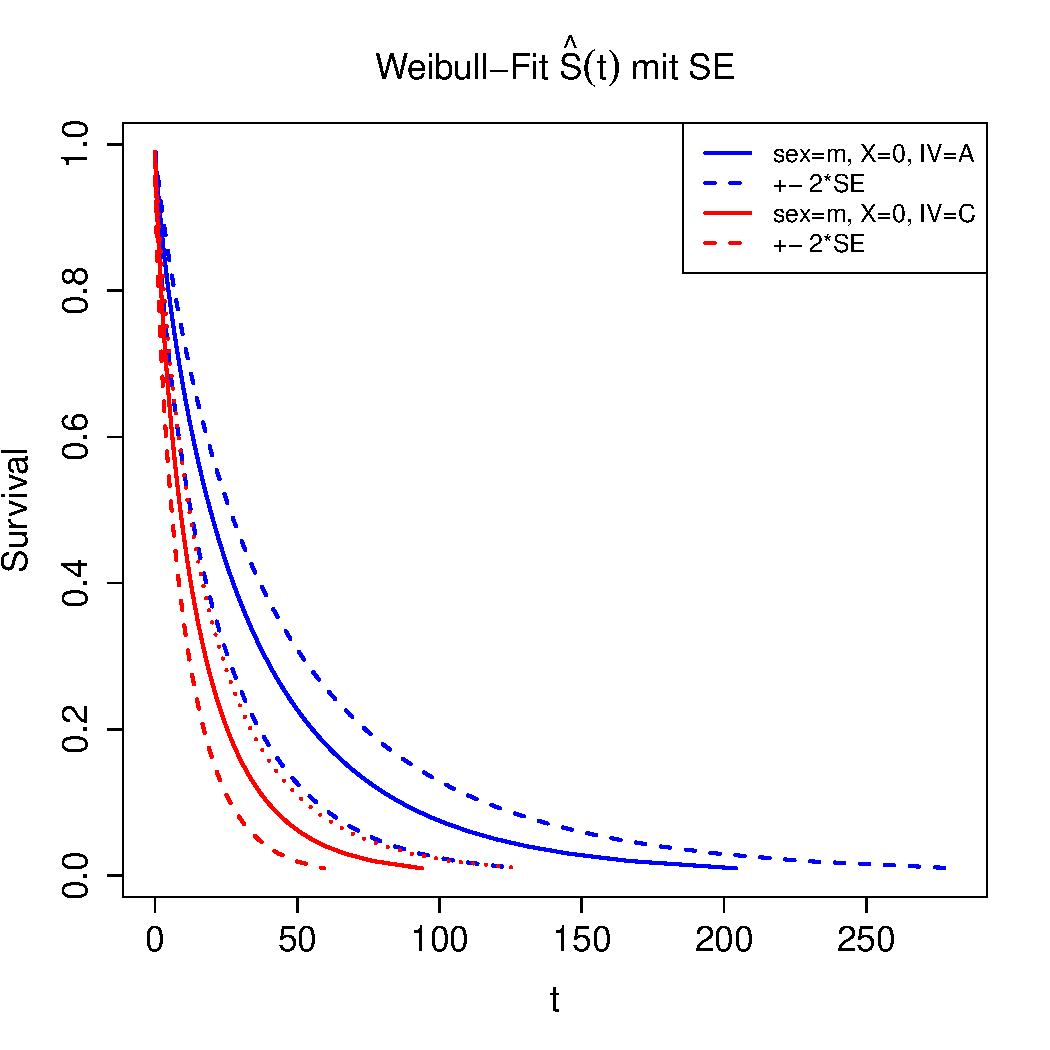
\includegraphics[width=8cm]{survivalWeib}
\vspace*{-1em}
\caption{Schätzung der Survival-Funktion $\hat{S}(t)$ aus Weibull-Modell für zwei männliche Personen mit Prädiktorwert $X=0$ aus Gruppe \lstinline!A! bzw.\ \lstinline!C!}
\label{fig:survivalWeib}
\end{figure}
